
\makeatletter
\@ifundefined{standalonetrue}{\newif\ifstandalone}{}
\@ifundefined{section}{\standalonetrue}{\standalonefalse}
\makeatother
\ifstandalone
\documentclass{report}

\usepackage{textcase}
%\usepackage{hyperref}
%\hypersetup{breaklinks=true}


% Added packages
\usepackage[usenames]{color}
\usepackage{amsfonts, amsmath, amssymb, graphics}

% NOTE: bibentry MUST appear before the hyperref or build will fail
\usepackage{bibentry}
\nobibliography*
\usepackage[square,sort,comma,numbers]{natbib}
  
\usepackage{float}
\usepackage[
	hidelinks,%
    %hyperindex=true,		% Make numbers of index links as well
   	backref=page, 		% Provide page listing where refs occur in the bibliography
	%breaklinks=true,
    %colorlinks,%
    %citecolor=green,%
    %filecolor=blue,%
    %linkcolor=red,%
    %urlcolor=red, 
]{hyperref}

\usepackage{dsfont}
%%%% USEPACKAGES for MACROS %%%%%
\usepackage{algpseudocode}
\usepackage[chapter]{algorithm}
%\usepackage{caption}
\usepackage{subcaption}
\usepackage{url}

\usepackage{array}
\usepackage{arydshln}
\usepackage{multirow}
\usepackage{multicol}
%\usepackage[section]{placeins}

\usepackage[usenames,dvipsnames]{color}
%\usepackage[english]{babel}
\usepackage{tabularx}
\usepackage{soul}
\usepackage{xparse}
\usepackage{listings}
%\usepackage[normalem]{ulem}



%%%%%%%%%%%%%%%
% Show a list of items "todo" or "done" 
% USAGE: 
% \begin{todolist} 
% 	\todo Something not finished
% 	\done Something finished
% \end{todolist} 
\newenvironment{todolist}{%
  \begin{list}{}{}% whatever you want the list to be
  \let\olditem\item
  \renewcommand\item{\olditem \textcolor{red}{(TODO)}: }
  \newcommand\todo{\olditem \textcolor{red}{(TODO)}: }
   \newcommand\done{\olditem \textcolor{ForestGreen}{(DONE)}: }
}{%
  \end{list}
} 
%%%%%%%%%%%%%%%

%%%%%%%%%%%%%%%
% Show a Author's Note
% USAGE: 
% \incomplete[Optional footnote message to further clarify note]{The text which is currently not finished}
\DeclareDocumentCommand \incomplete{ o m }
{%
\IfNoValueTF {#1}
{\textcolor{red}{Incomplete: \ul{#2}}} 
{\textcolor{red}{Incomplete: \ul{#2}}\footnote{Comment: #1}}%
}
%%%%%%%%%%%%%%%



%%%%%%%%%%%%%%%
% Show a Author's Note
% USAGE: 
% \authnote[Optional footnote message to further clarify note]{The note to your readers}
\DeclareDocumentCommand \authnote { o m }
{%
\IfNoValueTF {#1}
{\textcolor{blue}{Author's Note: \ul{#2}}} 
{\textcolor{blue}{Author's Note: \ul{#2}}\footnote{Comment: #1}}%
}
%%%%%%%%%%%%%%%



%%%%%%%%%%%%%%%
% Strike out text that doesn't belong in the paper
% USAGE: 
% \strike[Optional footnote to state why it doesn't belong]{Text to strike out}
\DeclareDocumentCommand \strike { o m }
{%
\setstcolor{Red}
\IfNoValueTF {#1}
{\textcolor{Gray}{\st{#2}}} 
{\textcolor{Gray}{\st{#2}}\footnote{Comment: #1}}%
}
%%%%%%%%%%%%%%%

\definecolor{light-gray}{gray}{0.95}

\newcommand{\cbox}[3]{
\ \\
\fcolorbox{#1}{#2}{
\parbox{\textwidth}{
#3
}
}
}

% Setup an environment similar to verbatim but which will highlight any bash commands we have
\lstnewenvironment{unixcmds}[0]
{
%\lstset{language=bash,frame=shadowbox,rulesepcolor=\color{blue}}
\lstset{ %
language=sh,		% Language
basicstyle=\ttfamily,
backgroundcolor=\color{light-gray}, 
rulecolor=\color{blue},
%frame=tb, 
columns=fullflexible,
%framexrightmargin=-.2\textwidth,
linewidth=0.8\textwidth,
breaklines=true,
%prebreak=/, 
  prebreak = \raisebox{0ex}[0ex][0ex]{\ensuremath{\hookleftarrow}},
%basicstyle=\footnotesize,       % the size of the fonts that are used for the code
%numbers=left,                   % where to put the line-numbers
%numberstyle=\footnotesize,      % the size of the fonts that are used for the line-numbers
%stepnumber=2,                   % the step between two line-numbers. If it's 1 each line 
                                % will be numbered
%numbersep=5pt,                  % how far the line-numbers are from the code
showspaces=false,               % show spaces adding particular underscores
showstringspaces=false,         % underline spaces within strings
showtabs=false,                 % show tabs within strings adding particular underscores
frame=single,	                % adds a frame around the code
tabsize=2,	                % sets default tabsize to 2 spaces
captionpos=b,                   % sets the caption-position to bottom
breakatwhitespace=false,        % sets if automatic breaks should only happen at whitespace
}
} { }

% Setup an environment similar to verbatim but which will highlight any bash commands we have
\lstnewenvironment{cppcode}[1]
{
%\lstset{language=bash,frame=shadowbox,rulesepcolor=\color{blue}}
\lstset{ %
	backgroundcolor=\color{light-gray}, 
	rulecolor=\color[rgb]{0.133,0.545,0.133},
	tabsize=4,
	language=[GNU]C++,
%	basicstyle=\ttfamily,
        basicstyle=\scriptsize,
        upquote=true,
        aboveskip={1.5\baselineskip},
        columns=fullflexible,
        %framexrightmargin=-.1\textwidth,
       %framexleftmargin=6mm,
        showstringspaces=false,
        extendedchars=true,
        breaklines=true,
        prebreak = \raisebox{0ex}[0ex][0ex]{\ensuremath{\hookleftarrow}},
        frame=single,
        showtabs=false,
        showspaces=false,
        showstringspaces=false,
        numbers=left,                   % where to put the line-numbers
	numberstyle=\footnotesize,      % the size of the fonts that are used for the line-numbers
	stepnumber=4,                   % the step between two line-numbers. If it's 1 each line 
                                % will be numbered
	firstnumber=#1,
         numbersep=5pt,                  % how far the line-numbers are from the code
        identifierstyle=\ttfamily,
        keywordstyle=\color[rgb]{0,0,1},
        commentstyle=\color[rgb]{0.133,0.545,0.133},
        stringstyle=\color[rgb]{0.627,0.126,0.941},
}
} { }

% Setup an environment similar to verbatim but which will highlight any bash commands we have
\lstnewenvironment{mcode}[1]
{
\lstset{ %
	backgroundcolor=\color{light-gray}, 
	rulecolor=\color[rgb]{0.133,0.545,0.133},
	tabsize=4,
	language=Matlab,
%	basicstyle=\ttfamily,
        basicstyle=\scriptsize,
        upquote=true,
        aboveskip={1.5\baselineskip},
        columns=fullflexible,
        %framexrightmargin=-.1\textwidth,
       %framexleftmargin=6mm,
        showstringspaces=false,
        extendedchars=true,
        breaklines=true,
        prebreak = \raisebox{0ex}[0ex][0ex]{\ensuremath{\hookleftarrow}},
        frame=single,
        showtabs=false,
        showspaces=false,
        showstringspaces=false,
        numbers=left,                   % where to put the line-numbers
	numberstyle=\footnotesize,      % the size of the fonts that are used for the line-numbers
	stepnumber=4,                   % the step between two line-numbers. If it's 1 each line 
                                % will be numbered
	firstnumber=#1,
         numbersep=5pt,                  % how far the line-numbers are from the code
        identifierstyle=\ttfamily,
        keywordstyle=\color[rgb]{0,0,1},
        commentstyle=\color[rgb]{0.133,0.545,0.133},
        stringstyle=\color[rgb]{0.627,0.126,0.941},
}
} { }

\newcommand{\inputmcode}[1]{%
\lstset{ %
	backgroundcolor=\color{light-gray},  %
	rulecolor=\color[rgb]{0.133,0.545,0.133}, %
	tabsize=4, %
	language=Matlab, %
%	basicstyle=\ttfamily,
        basicstyle=\scriptsize, %
        %        upquote=true,
        aboveskip={1.5\baselineskip}, %
        columns=fullflexible, %
        %framexrightmargin=-.1\textwidth,
       %framexleftmargin=6mm,
        showstringspaces=false, %
        extendedchars=true, %
        breaklines=true, %
        prebreak = \raisebox{0ex}[0ex][0ex]{\ensuremath{\hookleftarrow}}, %
        frame=single, %
        showtabs=false, %
        showspaces=false, %
        showstringspaces=false,%
        numbers=left,                   % where to put the line-numbers
	numberstyle=\footnotesize,      % the size of the fonts that are used for the line-numbers
	stepnumber=4,                   % the step between two line-numbers. If it's 1 each line 
                                % will be numbered
         numbersep=5pt,                  % how far the line-numbers are from the code
        identifierstyle=\ttfamily, %
        keywordstyle=\color[rgb]{0,0,1}, %
        commentstyle=\color[rgb]{0.133,0.545,0.133}, %
        stringstyle=\color[rgb]{0.627,0.126,0.941} %
}
\lstinputlisting{#1}%
}

%\lstset{ %
%	backgroundcolor=\color{light-gray}, 
%	rulecolor=\color[rgb]{0.133,0.545,0.133},
%	tabsize=4,
%	language=Matlab,
%%	basicstyle=\ttfamily,
%        basicstyle=\scriptsize,
%        upquote=true,
%        aboveskip={1.5\baselineskip},
%        columns=fullflexible,
%        %framexrightmargin=-.1\textwidth,
%       %framexleftmargin=6mm,
%        showstringspaces=false,
%        extendedchars=true,
%        breaklines=true,
%        prebreak = \raisebox{0ex}[0ex][0ex]{\ensuremath{\hookleftarrow}},
%        frame=single,
%        showtabs=false,
%        showspaces=false,
%        showstringspaces=false,
%        numbers=left,                   % where to put the line-numbers
%	numberstyle=\footnotesize,      % the size of the fonts that are used for the line-numbers
%	stepnumber=4,                   % the step between two line-numbers. If it's 1 each line 
%                                % will be numbered
%	firstnumber=#1,
%         numbersep=5pt,                  % how far the line-numbers are from the code
%        identifierstyle=\ttfamily,
%        keywordstyle=\color[rgb]{0,0,1},
%        commentstyle=\color[rgb]{0.133,0.545,0.133},
%        stringstyle=\color[rgb]{0.627,0.126,0.941},
%}


\newcommand{\Laplacian}[1]{\nabla^2 #1}

% set of all nodes received and contained on GPU
\newcommand{\setAllNodes}[0]{\mathcal{G}}
% set of stencil centers on GPU
\newcommand{\setCenters}[0]{\mathcal{Q}}
% set of stencil centers with nodes in \setDepend
\newcommand{\setBoundary}[0]{\mathcal{B}}
% set of nodes received by other GPUs
\newcommand{\setDepend}[0]{\mathcal{R}}
% set of nodes sent to other GPUs
\newcommand{\setProvide}[0]{\mathcal{O}}


\newcommand{\toprule}[0]{\hline}
\newcommand{\midrule}[0]{\hline\hline}
\newcommand{\bottomrule}[0]{\hline}

\newcolumntype{C}{>{\centering\arraybackslash}b{1in}}
\newcolumntype{L}{>{\flushleft\arraybackslash}b{1.5in}}
\newcolumntype{R}{>{\flushright\arraybackslash}b{1.5in}}
\newcolumntype{D}{>{\flushright\arraybackslash}b{2.0in}}
\newcolumntype{E}{>{\flushright\arraybackslash}b{1.0in}}

\DeclareSymbolFont{AMSb}{U}{msb}{m}{n}
\DeclareMathSymbol{\N}{\mathbin}{AMSb}{"4E}
\DeclareMathSymbol{\Z}{\mathbin}{AMSb}{"5A}
\DeclareMathSymbol{\R}{\mathbin}{AMSb}{"52}
\DeclareMathSymbol{\Q}{\mathbin}{AMSb}{"51}
\DeclareMathSymbol{\PP}{\mathbin}{AMSb}{"50}
\DeclareMathSymbol{\I}{\mathbin}{AMSb}{"49}
%\DeclareMathSymbol{\C}{\mathbin}{AMSb}{"43}

%%%%%% VECTOR NORM: %%%%%%%
\newcommand{\vectornorm}[1]{\left|\left|#1\right|\right|}
\newcommand{\vnorm}[1]{\left|\left|#1\right|\right|}
\newcommand{\by}[0]{\times}
\newcommand{\vect}[1]{\mathbf{#1}}
%\newcommand{\mat}[1]{\mathbf{#1}} 

%\renewcommand{\vec}[1]{ \textbf{#1} }
%%%%%%%%%%%%%%%%%%%%%%

%%%%%%% THM, COR, DEF %%%%%%%
%\newtheorem{theorem}{Theorem}[section]
%\newtheorem{lemma}[theorem]{Lemma}
%\newtheorem{proposition}[theorem]{Proposition}
%\newtheorem{corollary}[theorem]{Corollary}
%\newenvironment{proof}[1][Proof]{\begin{trivlist}
%\item[\hskip \labelsep {\bfseries #1}]}{\end{trivlist}}
%\newenvironment{definition}[1][Definition]{\begin{trivlist}
%\item[\hskip \labelsep {\bfseries #1}]}{\end{trivlist}}
%\newenvironment{example}[1][Example]{\begin{trivlist}
%\item[\hskip \labelsep {\bfseries #1}]}{\end{trivlist}}
%\newenvironment{remark}[1][Remark]{\begin{trivlist}
%\item[\hskip \labelsep {\bfseries #1}]}{\end{trivlist}}
%\newcommand{\qed}{\nobreak \ifvmode \relax \else
%      \ifdim\lastskip<1.5em \hskip-\lastskip
%      \hskip1.5em plus0em minus0.5em \fi \nobreak
%      \vrule height0.75em width0.5em depth0.25em\fi}
%%%%%%%%%%%%%%%%%%%%%%

%
%\usepackage[algochapter]{algorithm2e}
%\usepackage[usenames]{color}
% colors to show the corrections
\newcommand{\red}[1]{\textbf{\textcolor{red}{#1}}}
\newcommand{\blue}[1]{\textbf{\textcolor{blue}{#1}}}
\newcommand{\cyan}[1]{\textbf{\textcolor{cyan}{#1}}}
\newcommand{\green}[1]{\textbf{\textcolor{green}{#1}}}
\newcommand{\magenta}[1]{\textbf{\textcolor{magenta}{#1}}}
\newcommand{\orange}[1]{\textbf{\textcolor{orange}{#1}}}
%%%%%%%%%% DK DK
% comments between authors
\newcommand{\toall}[1]{\textbf{\green{@@@ All: #1 @@@}}}
\newcommand{\toevan}[1]{\textbf{\red{*** Evan: #1 ***}}}
%\newcommand{\toevan}[1]{}  % USE FOR FINAL VERSION
\newcommand{\toe}[1]{\textbf{\red{*** Evan: #1 ***}}}
\newcommand{\tog}[1]{\textbf{\blue{*** Gordon: #1 ***}}}
%\newcommand{\togordon}[1]{\textbf{\blue{*** Gordon: #1 ***}}}
\renewcommand{\ge}[3]{{\textcolor{blue}{*** \textbf{Gordon:}\strike{#1} #2 ***}}\red{(#3)}}
\renewcommand{\ge}[3]{{\textcolor{blue}{#2}}}
\renewcommand{\ge}[3]{{\textcolor{Red}{#2}}}
\newcommand{\eb}[3]{{\textcolor{Red}{*** \textbf{Evan:}\strike{#1} #2 ***}}\red{(#3)}}
\renewcommand{\eb}[3]{{{\textcolor{Red}{#2}}}}
%\def\ge#1#2#3{}{\textbf{\blue{*** Gordon: #2 ***}}}{(#3)}
\newcommand{\gee}[1]{{\bf{\blue{{\em #1}}}}}
\newcommand{\old}[1]{}
\newcommand{\del}[1]{***#1*** }



% \DeclareMathOperator{\Sample}{Sample}
%\let\vaccent=\v % rename builtin command \v{} to \vaccent{}
%\renewcommand{\vec}[1]{\ensuremath{\mathbf{#1}}} % for vectors
\newcommand{\gv}[1]{\ensuremath{\mbox{\boldmath$ #1 $}}} 
% for vectors of Greek letters
\newcommand{\uv}[1]{\ensuremath{\mathbf{\hat{#1}}}} % for unit vector
\newcommand{\abs}[1]{\left| #1 \right|} % for absolute value
\newcommand{\avg}[1]{\left< #1 \right>} % for average
\let\underdot=\d % rename builtin command \d{} to \underdot{}
\renewcommand{\d}[2]{\frac{d #1}{d #2}} % for derivatives
\newcommand{\dd}[2]{\frac{d^2 #1}{d #2^2}} % for double derivatives
\newcommand{\pd}[2]{\frac{\partial #1}{\partial #2}} 
% for partial derivatives
\newcommand{\pdd}[2]{\frac{\partial^2 #1}{\partial #2^2}} 
\newcommand{\pdda}[3]{\frac{\partial^2 #1}{\partial #2 \partial #3}} 
% for double partial derivatives
\newcommand{\pdc}[3]{\left( \frac{\partial #1}{\partial #2}
 \right)_{#3}} % for thermodynamic partial derivatives
\newcommand{\ket}[1]{\left| #1 \right>} % for Dirac bras
\newcommand{\bra}[1]{\left< #1 \right|} % for Dirac kets
\newcommand{\braket}[2]{\left< #1 \vphantom{#2} \right|
 \left. #2 \vphantom{#1} \right>} % for Dirac brackets
\newcommand{\matrixel}[3]{\left< #1 \vphantom{#2#3} \right|
 #2 \left| #3 \vphantom{#1#2} \right>} % for Dirac matrix elements
\newcommand{\grad}[1]{\gv{\nabla} #1} % for gradient
\let\divsymb=\div % rename builtin command \div to \divsymb
\renewcommand{\div}[1]{\gv{\nabla} \cdot #1} % for divergence
\newcommand{\curl}[1]{\gv{\nabla} \times #1} % for curl
\let\baraccent=\= % rename builtin command \= to \baraccent
\renewcommand{\=}[1]{\stackrel{#1}{=}} % for putting numbers above =
\newcommand{\diffop}[1]{\mathcal{L}#1}
\newcommand{\boundop}[1]{\mathcal{B}#1}
\newcommand{\rvec}[0]{{\bf r}}

\newcommand{\Interior}[0]{\Omega}
\newcommand{\domain}[0]{\Omega}
%\newcommand{\Boundary}[0]{\partial \Omega}
\newcommand{\Boundary}[0]{\Gamma}

\newcommand{\on}[1]{\hskip1.5em \textrm{ on } #1}

\newcommand{\gemm}{\texttt{GEMM}}
\newcommand{\trmm}{\texttt{TRMM}}
\newcommand{\gesvd}{\texttt{GESVD}}
\newcommand{\geqrf}{\texttt{GEQRF}}


\newcommand{\minitab}[2][l]{\begin{tabular}{#1}#2\end{tabular}}
\newcommand{\comm}[1]{\textcolor{red}{\textit{#1}}}

\newcommand{\nfrac}[2]{
\nicefrac{#1}{#2}
%\frac{#1}{#2}
}

\usepackage{xparse}
\usepackage{soul}


%%%%%%%%%%%%%%%
% Show a Author's Note
% USAGE: 
% \incomplete[Optional footnote message to further clarify note]{The text which is currently not finished}
\DeclareDocumentCommand \incomplete{ o m }
{%
\IfNoValueTF {#1}
{\textcolor{red}{Incomplete: \ul{#2}}} 
{\textcolor{red}{Incomplete: \ul{#2}}\footnote{Comment: #1}}%
}
%%%%%%%%%%%%%%%



%%%%%%%%%%%%%%%
% Show a Author's Note
% USAGE: 
% \authnote[Optional footnote message to further clarify note]{The note to your readers}
\DeclareDocumentCommand \authnote { o m }
{%
\IfNoValueTF {#1}
{\textcolor{blue}{Author's Note: \ul{#2}}} 
{\textcolor{blue}{Author's Note: \ul{#2}}\footnote{Comment: #1}}%
}
%%%%%%%%%%%%%%%



%%%%%%%%%%%%%%%
% Strike out text that doesn't belong in the paper
% USAGE: 
% \strike[Optional footnote to state why it doesn't belong]{Text to strike out}
\DeclareDocumentCommand \strike { o m }
{%
\setstcolor{red}
\IfNoValueTF {#1}
{\textcolor{Gray}{\st{#2}}} 
{\textcolor{Gray}{\st{#2}}\footnote{Comment: #1}}%
}
%%%%%%%%%%%%%%%



%
% colors to show the corrections
\newcommand{\red}[1]{\textbf{\textcolor{red}{#1}}}
\newcommand{\blue}[1]{\textbf{\textcolor{blue}{#1}}}
\newcommand{\cyan}[1]{\textbf{\textcolor{cyan}{#1}}}
\newcommand{\green}[1]{\textbf{\textcolor{green}{#1}}}
\newcommand{\magenta}[1]{\textbf{\textcolor{magenta}{#1}}}
\newcommand{\orange}[1]{\textbf{\textcolor{orange}{#1}}}
%%%%%%%%%% DK DK
% comments between authors
\newcommand{\toall}[1]{\textbf{\green{@@@ All: #1 @@@}}}
\newcommand{\toevan}[1]{\textbf{\red{*** Evan: #1 ***}}}
%\newcommand{\toevan}[1]{}  % USE FOR FINAL VERSION
\newcommand{\toe}[1]{\textbf{\red{*** Evan: #1 ***}}}
\newcommand{\tog}[1]{\textbf{\blue{*** Gordon: #1 ***}}}
%\newcommand{\togordon}[1]{\textbf{\blue{*** Gordon: #1 ***}}}
\renewcommand{\ge}[3]{{\textcolor{blue}{*** \textbf{Gordon:}\strike{#1} #2 ***}}\red{(#3)}}
\renewcommand{\ge}[3]{{\textcolor{blue}{#2}}}
\renewcommand{\ge}[3]{{\textcolor{red}{#2}}}
\newcommand{\eb}[3]{{\textcolor{red}{*** \textbf{Evan:}\strike{#1} #2 ***}}\red{(#3)}}
\renewcommand{\eb}[3]{{{\textcolor{red}{#2}}}}
%\def\ge#1#2#3{}{\textbf{\blue{*** Gordon: #2 ***}}}{(#3)}
\newcommand{\gee}[1]{{\bf{\blue{{\em #1}}}}}
\newcommand{\old}[1]{}
\newcommand{\del}[1]{***#1*** }



% Rename  this file          misc_mac.tex
%----------------------------------------------------------------------
%%%%%%%%%%%%%%%%%%%%%%%%%%%%%%%%%%%%%%%%%%%%%%%%%%%%%%%%%%%%%%%%%%%%%%%%%%%%%%%
%
%	Math Symbols   Math Symbols   Math Symbols   Math Symbols   
%
%%%%%%%%%%%%%%%%%%%%%%%%%%%%%%%%%%%%%%%%%%%%%%%%%%%%%%%%%%%%%%%%%%%%%%%%%%%%%%%
\def\pmb#1{\setbox0=\hbox{$#1$}%
	\kern-.025em\copy0\kern-\wd0
	\kern.05em\copy0\kern-\wd0
	\kern-.025em\raise.0433em\box0}
\def\pmbf#1{\pmb#1}
\def\bfg#1{\pmb#1}

% BETTER VALUES FOR AUTOMATIC FIGURE PLACEMENT THAN THOSE PROVIDED BY 
% LATEX DEFAULTS.

\renewcommand{\textfloatsep}{1ex}
\renewcommand{\floatpagefraction}{0.9}
\renewcommand{\intextsep}{1ex}
\renewcommand{\topfraction}{.9}
\renewcommand{\bottomfraction}{.9}
\renewcommand{\textfraction}{.1}

% #1  position of floating figure (h|t|b|p)
% #1  EPS postscript file
% #2  size
% #3  caption

%usage of newfig:
%  \newfig{file.ps}{3in}{Fig1: this is a figure}

\input{epsf}
\def\newfig#1#2#3{
  \begin{figure}[htbp]
  \vspace{1ex}
  \setlength{\epsfxsize}{#2}
  \centerline{\epsfbox{#1}}
  \vspace{-.1in}\caption{\small #3}\break\vspace{.2in}
  \label{#1}
  \end{figure}
}

%usage of newfigtwo: 2 figures, vertically stacked
% \newfig
%	{file1.ps}
%	{file2.ps}
%	{width}
%	{vertical space}
%	{Caption}

\def\newfigtwo#1#2#3#4#5{
  \begin{figure}[htbp]
  \vspace{1ex}
  \setlength{\epsfxsize}{#3}
  \centerline{\epsfbox{#1}}
  \vspace{#4}
  \setlength{\epsfxsize}{#3}
  \centerline{\epsfbox{#2}}
  \vspace{-.1in}\caption{\small #5}\break\vspace{.2in}
  \label{#1}
  \end{figure}
}

\def\newfigh#1#2#3#4{  % add height specification
  \begin{figure}[htbp]
  \vspace{1ex}
  \setlength{\epsfxsize}{#2}
  \setlength{\epsfysize}{#4}
  \centerline{\epsfbox{#1}}
  \vspace{-.1in}\caption{\small #3}\break\vspace{.2in}
  \label{#1}
  \end{figure}
}

\def\herefig#1#2#3{
  \begin{figure}[h]
  \setlength{\epsfxsize}{#2}
  \centerline{\epsfbox{#1}}
  \caption{\small #3}
  \label{#1}
  \end{figure}
}

\def\etal{{{\em et~al.\,\,}}}
\def\note#1{\\ =====#1===== \\}
\def\FBOX#1{\ \\ \fbox{\begin{minipage}{5in}#1\end{minipage}}\\ }
\newcount\sectionno     \sectionno=0
\newcount\eqnum         \eqnum=0
\def\addeqno{\global\advance \eqnum by  1 }
\def\subeqno{\global\advance \eqnum by -1 }
%\def\eqn{\addeqno \eqno \hbox{(\number\sectionno.\number\eqnum)} }

\def\tildetilde#1{\tilde{\tilde{#1}}}
\def\barbar#1{\overbar{\overbar{#1}}}

\def\vsp#1{\vspace{#1 ex}}
\def\fpar{\hspace{\parindent}}
%
%  \pf : 2 arguments: numerator and denominator of partial derivative
%
\def\pf#1#2{{\frac{\partial{#1}}{\partial{#2}}}}
\def\pfs#1#2{{\partial_{#2}{#1}}}
\def\pftwo#1#2{{\frac{\partial^2{#1}}{\partial{#2}^2}}}
\def\pfxx#1#2{{\frac{\partial^2{#1}}{\partial{#2}^2}}}
%\def\pfxy#1#2{{\frac{\partial^2{#1}}{\partial{#2}\partial{#3}}}}
\def\pfn#1#2#3{{\frac{\partial^{#1}{#2}}{\partial{#3}^{#1}}}}
\def\df#1#2{{\frac{d{#1}}{d{#2}}}}
\def\dfn#1#2#3{{\frac{d^{#1}{#2}}{d{#3}^{#1}}}}
\def\Dt#1#2{\frac{D#1}{D#2}}
\def\dt#1#2{\frac{d#1}{d#2}}
\def\bld#1{{\bf #1}}
\def\pfp#1#2#3{\pf{}{#3}{\left(\frac{#1}{#2}\right)}}

\def\norm#1{\|#1\|}

%
% Graphic characters  (\dot already defined by TeX/LateX)
%
\def\dash{\rule[1.5pt]{2mm}{.3mm}\HS{.9mm}}
\def\dott{\rule[1.5pt]{.7mm}{.3mm}\HS{.7mm}}
\def\dashline{\dash\dash\dash}
\def\dotline{\dott\dott\dott\dott\dott\dott}
\def\dashdotline{\dash$\cdot$\HS{.9mm}\dash}
\def\solidline{\rule[2pt]{7mm}{.3mm}}
% 
% overcircle
%
\def\ovcircle#1{\buildrel{\circ}\over{#1}}
%\def\below#1#2{\buildrel{#2}\under{#1}}
%\def\above#1#2{\buildrel{#2}\over{#1}}
%
%  big parenthesis and brackets
%
\def\bigpar#1#2{{\left(\frac{#1}{#2}\right)}}
\def\bigbra#1#2{{\left\[\frac{#1}{#2}\right\]}}

\def\Lp{\left(}
\def\Rp{\right)}
\def\Lb{\left[}
\def\Rb{\right]}
\def\Ln{\left\langle}
\def\Rn{\right\rangle}
\def\Ld{\left.}
\def\Rd{\right.}
\def\Lv{\left|}
\def\Rv{\right|}
\def\Lbr{\left|}
\def\Rbr{\right|}
\def\lng{\langle}
\def\rng{\rangle}
\def\Lc{\left\{}
\def\Rc{\right\}}
%%% %

% Cannot be handled by Lyx
%\def\[{{[}}
%\def\]{{]}}

%
\def\eol{\nonumber \\}
\def\eolnonb{\nonumber\\}
\def\eolnb{\\}
\def\nonb{\nonumber}
\def\be{\begin{equation}}
\def\ee{\end{equation}}
\def\BEQNA{\begin{eqnarray}}
\def\EEQNA{\end{eqnarray}}
\def\eqa{&=&}
\def\beqna{\begin{eqnarray}}
\def\eeqna{\end{eqnarray}}
\def\bverb{\begin{verbatim}}
\def\everb{\end{verbatim}}
\def\VERB#1{\bverb #1 \everb}
\def\btbl{\begin{tabular}}
\def\etbl{\end{tabular}}
\def\bmini{\begin{minipage}[t]{5.5in}}
\def\emini{\end{minipage}}
\def\parray#1#2{\left(\begin{array}{#1}#2\end{array}\right)}
\def\barray#1#2{\left[\begin{array}{#1}#2\end{array}\right]}
\def\carray#1#2{\left\{\begin{array}{#1}#2\end{array}\right.}
\def\darray#1#2{\left|\begin{array}{#1}#2\end{array}\right|}

\def\BEGTABLE#1{\begin{table}[hbt]\vspace{2ex}\begin{center}\bmini\centering\btbl{#1}}
\def\ENDTABLE#1#2{\etbl\caption[#1]{#2}\EMINI\end{center}\vspace{2ex}\end{table}}

\def\bfltbl#1{\begin{table}[hbt]\vspace{2ex}\begin{center}\bmini\centering\btbl{#1}}
\def\efltbl#1#2{\etbl\caption[#1]{#2}\emini\end{center}\vspace{2ex}\end{table}}
\def\mcol{\multicolumn}
%
%  label equations with (#)
%
\def\reff#1{(\ref{#1})}
%
%  macros borrowed from viewgraph package
%

\newenvironment{LETTRS}[3]{\begin{letter}{#1}
\input{origin}\opening{Dear #2:}\input{#3}\closing{Sincerely yours,}\end{letter}}{\clearpage}

\newenvironment{VIEW}[1]{{\BC\Huge\bf #1 \EC}\LARGE\VS{.05in}}{\clearpage}

\def\RM#1{\rm{#1\ }}
\def\BV{\begin{VIEW}}
\def\EV{\end{VIEW}}

\def\NI{\noindent}

\def\VS{\vspace*}
\def\HS{\hspace*}
\def\IT{\item}

\def\BARR{\begin{array}}
\def\EARR{\end{array}}

\def\BPARR{\left(\begin{array}}
\def\EPARR{\end{array}\right)}

\def\BDET{\left|\begin{array}}
\def\EDET{\end{array}\right|}

\def\BDF{\begin{definition}}
\def\EDF{\end{definition}}

\def\BSU{\begin{block}{Summary}}
\def\ESU{\end{block}}

\def\BEX{\begin{example}}
\def\EEX{\end{example}}

\def\BTH{\begin{theorem}}
\def\ETH{\end{theorem}}

\def\BCO{\begin{corollary}}
\def\ECO{\end{corollary}}

\def\BPROOF{\begin{proof}}
\def\EPROOF{\end{proof}}

\def\BLM{\begin{lemma}}
\def\ELM{\end{lemma}}

\def\BEQ{\begin{equation}}
\def\EEQ{\end{equation}}

\def\BEQNNB{$$}
\def\EEQNNB{$$}

\def\BE{\begin{enumerate}}
\def\EE{\end{enumerate}}

\def\BD{\begin{description}}
\def\ED{\end{description}}

\def\BI{\begin{itemize}}
\def\EI{\end{itemize}}

\def\BC{\begin{center}}
\def\EC{\end{center}}

\def\BFIG{\begin{figure}}
\def\EFIG{\end{figure}}

\def\BTABB{\begin{tabbing}}
\def\ETABB{\end{tabbing}}

\def\BMINI{\begin{minipage}}
\def\EMINI{\end{minipage}}

\def\BTABLE{\begin{table}}
\def\ETABLE{\end{table}}

\def\BTABUL{\begin{tabular}}
\def\ETABUL{\end{tabular}}

\def\MCOL{\multicolumn}
\def\UL{\underline}
\def\ULL#1{\UL{\UL{#1}}}

\def\BDOC{\begin{document}}
\def\EDOC{\end{document}}

\def\EM#1{{\em #1\/}}
\def\FN{\footnote}

% Courtesy of Ugo Piomelli

\def\latexfig #1 #2 #3 #4 #5 {\ \vfill
\hfill\hbox to 0.05in{\vbox to #3truein{
         \special{psfile="#1" angle=270 hscale=100 
                  hoffset=#4 voffset=#5 vscale=100} }\hfill}
\hfill\vspace{-0.1in}        }

% #1 is the .ps filename
% #2 is not used in the present version
% #3 is the size of the white space left above the caption (in inches)
% #4 is the horizontal offset from some unknown reference point.
%    It is in 1/72 of an inch and is positive to the right.
% #5 is the vertical offset from some unknown reference point.
%    It is in 1/72 of an inch and is positive upwards.


\newcommand{\mathsym}[1]{{}}
\newcommand{\unicode}[1]{{}}
\newcommand{\ep}{\epsilon}
\newcommand{\vv}{\mathbf{v}}
\newcommand{\vu}{\mathbf{u}}
\newcommand{\vx}{\mathbf{x}}

\newcommand{\Laplacian}[1]{\nabla^2 #1}
\newcommand{\LaplaceBeltrami}[1]{\Delta_S #1}

% set of all nodes received and contained on GPU
\newcommand{\setAllNodes}[0]{\mathcal{G}}
% set of stencil centers on GPU
\newcommand{\setCenters}[0]{\mathcal{Q}}
% set of stencil centers with nodes in \setDepend
\newcommand{\setBoundary}[0]{\mathcal{B}}
% set of nodes received by other GPUs
\newcommand{\setDepend}[0]{\mathcal{R}}
% set of nodes sent to other GPUs
\newcommand{\setProvide}[0]{\mathcal{O}}





\usepackage{tabularx} 
\newcolumntype{C}{>{\centering\arraybackslash}b{1in}}
\newcolumntype{L}{>{\flushleft\arraybackslash}b{1.5in}}
\newcolumntype{R}{>{\flushright\arraybackslash}b{1.5in}}
\newcolumntype{D}{>{\flushright\arraybackslash}b{2.0in}}
\newcolumntype{E}{>{\flushright\arraybackslash}b{1.0in}}


 


%\usepackage{xcolor}

%\usepackage{refcheck}
% Sepia
%\definecolor{myBGcolor}{HTML}{F6F0D6}
%\definecolor{myTextcolor}{HTML}{4F452C}
% Dark
%\definecolor{myBGcolor}{HTML}{3E3535}
%\definecolor{myTextcolor}{HTML}{CFECEC}
%\color{myTextcolor}
%\pagecolor{myBGcolor}
 
\usepackage[margin=1.25in]{geometry}

\begin{document}
\fi


\chapter{Distributed RBF-FD}
\label{chap:distributed_rbffd}

Parallelizing applications in a distributed computing environment requires three
design decisions \cite{Saad2003}: 
\begin{enumerate} 
\item Partition the problem to distribute work across multiple processes. Intelligent partitioning
impacts load balancing and communication latency.
\item Determine the subset of node information,
solution values, etc. that are visible to each process, and establish index mappings that translate between a local context and the global problem. 
\item Establish a local ordering of data. The right local order can improve solver performance and/or simplify data movement. %Of particular interest here is how to minimize data movement at each iteration. In Chapter~\ref{chap:multigpu_rbffd} the local ordering will help minimize data transfer between CPU and GPU. 
\end{enumerate}

This chapter details the first implementation of RBF-FD designed for distributed computing environments and a few optimizations that help scale computation across a thousand processes. The discussion in this chapter applies to both multi-CPU and multi-GPU implementations of RBF-FD. Since each GPU is used as an accelerator, details of partitioning, local and global index mappings, and node ordering are managed on the CPU.  

We operate under the assumption that inter-process communication is managed by the \emph{Message Passing Interface (MPI)} \cite{MPI}. Detail on how communication collectives are used is included below in Section~\ref{sec:mpi_collectives}. We use the term \emph{MPI process} to refer to a process that occupies one CPU core and is associated with at most one GPU accelerator. MPI processes on multiple cores of the same CPU behave the same as processes on independent compute nodes in a cluster; the only difference being the fabric used for communication (i.e., fast shared memory versus a slower QDR InfiniBand). MPI always uses the fastest interconnect possible to connect processes. 

In order to manage expectations of how well the code will run in a distributed environment, we turn to Amdahl's law, which states that the total speedup possible for $p$ processors is limited by the fraction of code that must run in serial \cite{Shi2012}:
\begin{align}
S_p = \frac{T_s + T_p}{T_s + \frac{T_p}{p}},  \nonumber
\end{align}
where $T_s$ and $T_p$ are the time spent in serial and parallelizable portions of code respectively. Amdahl's law reveals that scaling to a large number of processors, $p$, can make the time in parallelizable portions of code vanish, but $T_s$ is constant. Communication is always included in $T_s$, so it is pertinent to minimize the cost of communication for maximum gain. Our initial implementation of distributed RBF-FD on multiple CPUs and multiple GPUs (\cite{BolligFlyerErlebacher2012}) had an extremely high cost of communication, which limited parallel execution to only a dozen or so processes. This chapter details the design and tuning of a distributed RBF-FD implementation capable of scaling across more than a thousand processors. 




%TODO: related distributed 
%TODO: \authnote{finish additional related work}
%The power of hindsight reveals that RBF-FD can be implemented with any library designed for sparse matrix algebra. 
%Our implementation is unlikely to to compete well against a number of well established libraries that have seen decades of active development. 
% that PETSc, Hypre, Trilinos are all libraries/frameworks that we could have developed in, but none of them had GPU support. We continued with custom built code, but that decision required additional decisions from us. 

%\cite{Yokota2010}
%\cite{Yokota2012}
%\cite{Schubert2011} 

%TODO: Similar Overlapping algorithm: \url{http://arxiv.org/pdf/1101.0091v1.pdf}
 %Imbalanced computation can be the source of excessive delays as processors sit idle and wait for other processors to catch up. 




\section{Partitioning}

Parallelization of RBF-FD relies on \emph{domain decomposition}. Domain decomposition methods simply subdivide/partition the computational domain of a PDE into \emph{subdomains}, which are then solved independently. Subdomains can be solved sequentially by the same MPI process or in parallel across multiple processes. A number of methods exist for domain decomposition including Multiplicative Schwarz, Additive Schwarz, and Restricted Additive Schwarz (see related works in \cite{Yokota2010,StCyr2007}). The choice of method determines how the domain is subdivided, and how often data is passed between subdomains (i.e., how parallelizable the method is). Domain decomposition methods are well known as a form of preconditioning (see e.g., \cite{Beatson2000, StCyr2007}), but the two Additive variants of Schwarz decomposition are inherently parallel and naturally extend to distributed architectures \cite{Yokota2010, Gropp1990}. 

The parallelization strategy employed for RBF-FD in this work is equivalent to a Restricted Additive Schwarz (RAS), although our strategy was implemented prior to formal knowledge of the RAS method. In this case we assume that partitioning occurs within the spatial domain. At each time-step the PDE is first solved independently within subdomains, and then information is shared across subdomain boundaries to ensure a consistent global solution entering the next time-step. We also assume that subdomains are always assigned to independent processes, even though each process could operate on multiple subdomains in theory. 

Following the notation in \cite{StCyr2007}, consider domain, $\Interior$, decomposed into overlapping subdomains $\Interior_1$ and $\Interior_2$, with a global boundary $\Boundary = \Boundary_1 \cup \Boundary_2$. At each time-step we seek the simultaneous solution to
\begin{center}
\begin{minipage}{0.4\linewidth}
\begin{align*}
\diffop{u_{1}^{n+1}} & = f \ \ \text{ in }\Interior_1,\\
\boundop{u_{1}^{n+1}} &= g \ \ \text{ on }\Boundary_1, \\
u_{1}^{n+1} & = u_2^{n} \ \ \text{ on }\Gamma_{12}, 
\end{align*}
\end{minipage}
\begin{minipage}{0.4\linewidth} 
\begin{align}
\diffop{u_{2}^{n+1}} & = f \ \ \text{ in }\Interior_2 \nonumber \\
\boundop{u_{2}^{n+1}} & = g \ \ \text{ on }\Boundary_2, \label{eq:rasm_example} \\
u_{2}^{n+1} & = u_1^{n} \ \ \text{ on }\Gamma_{21},  \nonumber
\end{align}
\end{minipage}
\end{center}
\ 

\noindent where $\Gamma_{ij}$ indicates overlap between subdomains and is read as the subset of subdomain $j$ required by subdomain $i$ (i.e., $\Gamma_{ij} = \Boundary_i \cap \Interior_j$). A Dirichlet boundary condition connects subdomains at the interfaces. Although not considered here, future investigations may find Robin-type conditions of interest due to their convergence accelerating properties in the context of Schwarz methods for elliptic PDEs (\cite{StCyr2007}). 

Equation~\ref{eq:rasm_example} illustrates how nicely a PDE can be split in half, and then solved by independent processes. To enforce the Dirichlet conditions on $\Gamma_{ij}$, MPI transfers values $u_j^{n}$ across interfaces at each time-step. Note that as the number of subdomains increases, additional constraints for $\Gamma_{ij}$ must be imposed on each subdomain. The worst case a partitioning for $p$ subdomains requires $p-1$ conditions (i.e., $\Gamma_{ij}$, for $i,j=1,2,...,p$ and $i \neq j$). Ideally each $\Interior_i$ should only overlap with a small number of neighboring subdomains to minimize MPI communication. 


The continuous form of decomposition in Equation~\ref{eq:rasm_example} allows complete freedom in choosing how subdomains are actually partitioned. In this work we assume partitioning of the geometry on which the PDE is solved. Of particular interest here is how to partition the unit sphere, but the challenge of more general geometries is also kept in mind. 

For ease of development and parallel debugging, partitioning is initially
assumed to be linear along one spatial dimension (in this case the $x$-axis). Each partition/subdomain is then contiguous and overlaps with neighboring subdomains to the left and right. This approach is not uncommon when solving PDEs on rectangular domains (see e.g., \cite{Divo2007, Thibault2009}). 

% A similar decomposition occurs in \cite{Divo2007} where the authors apply a local RBF collocation scheme to model viscous flow and heat transfer on rectangular domains. Thibault and Senocak  \cite{Thibault2009} partition a rectangular domain along the $z$-dimension for a variety of 3-D fluid benchmarks. 

Figure~\ref{fig:decomposed_sphere} illustrates the partitioning of
$N=10,201$ nodes on the unit sphere for four processes. 
Each partition, illustrated as a unique color, contains many stencil centers.  
A center's coordinates easily identify the containing partition. In cases where stencils in one partition depend on stencil nodes in another, we say that the dependencies (i.e., the nodes in $\Gamma_{ij}$) are \emph{ghost nodes}. 
In many ways ghost nodes are treated the same as any other stencil node. The MPI process in charge of a partition is fully aware of the ghost node coordinate, current solution value(s), etc. However, ghost nodes are managed by another subdomain/process, so changes must be explicitly synchronized in order to maintain consistency. 

Alternating representations between node points and interpolated surfaces in Figure~\ref{fig:decomposed_sphere} illustrates the
overlap regions where ghost nodes reside. Due to stencil dependencies, the representations of overlap regions are double-wide---i.e., they contain a set of ghost nodes for both the left and right partitions. The illustrated width of the overlap is between five and six nodes. As the stencil size increases, the overlap grows as $\sqrt{n}$. Since stencils need not have symmetric dependencies (i.e., if stencil $s_1$ depends on $s_2$, $s_2$ need not depend on $s_1$), the number of ghost nodes for each partition can vary. 

\begin{figure}[ht!]
\begin{center}
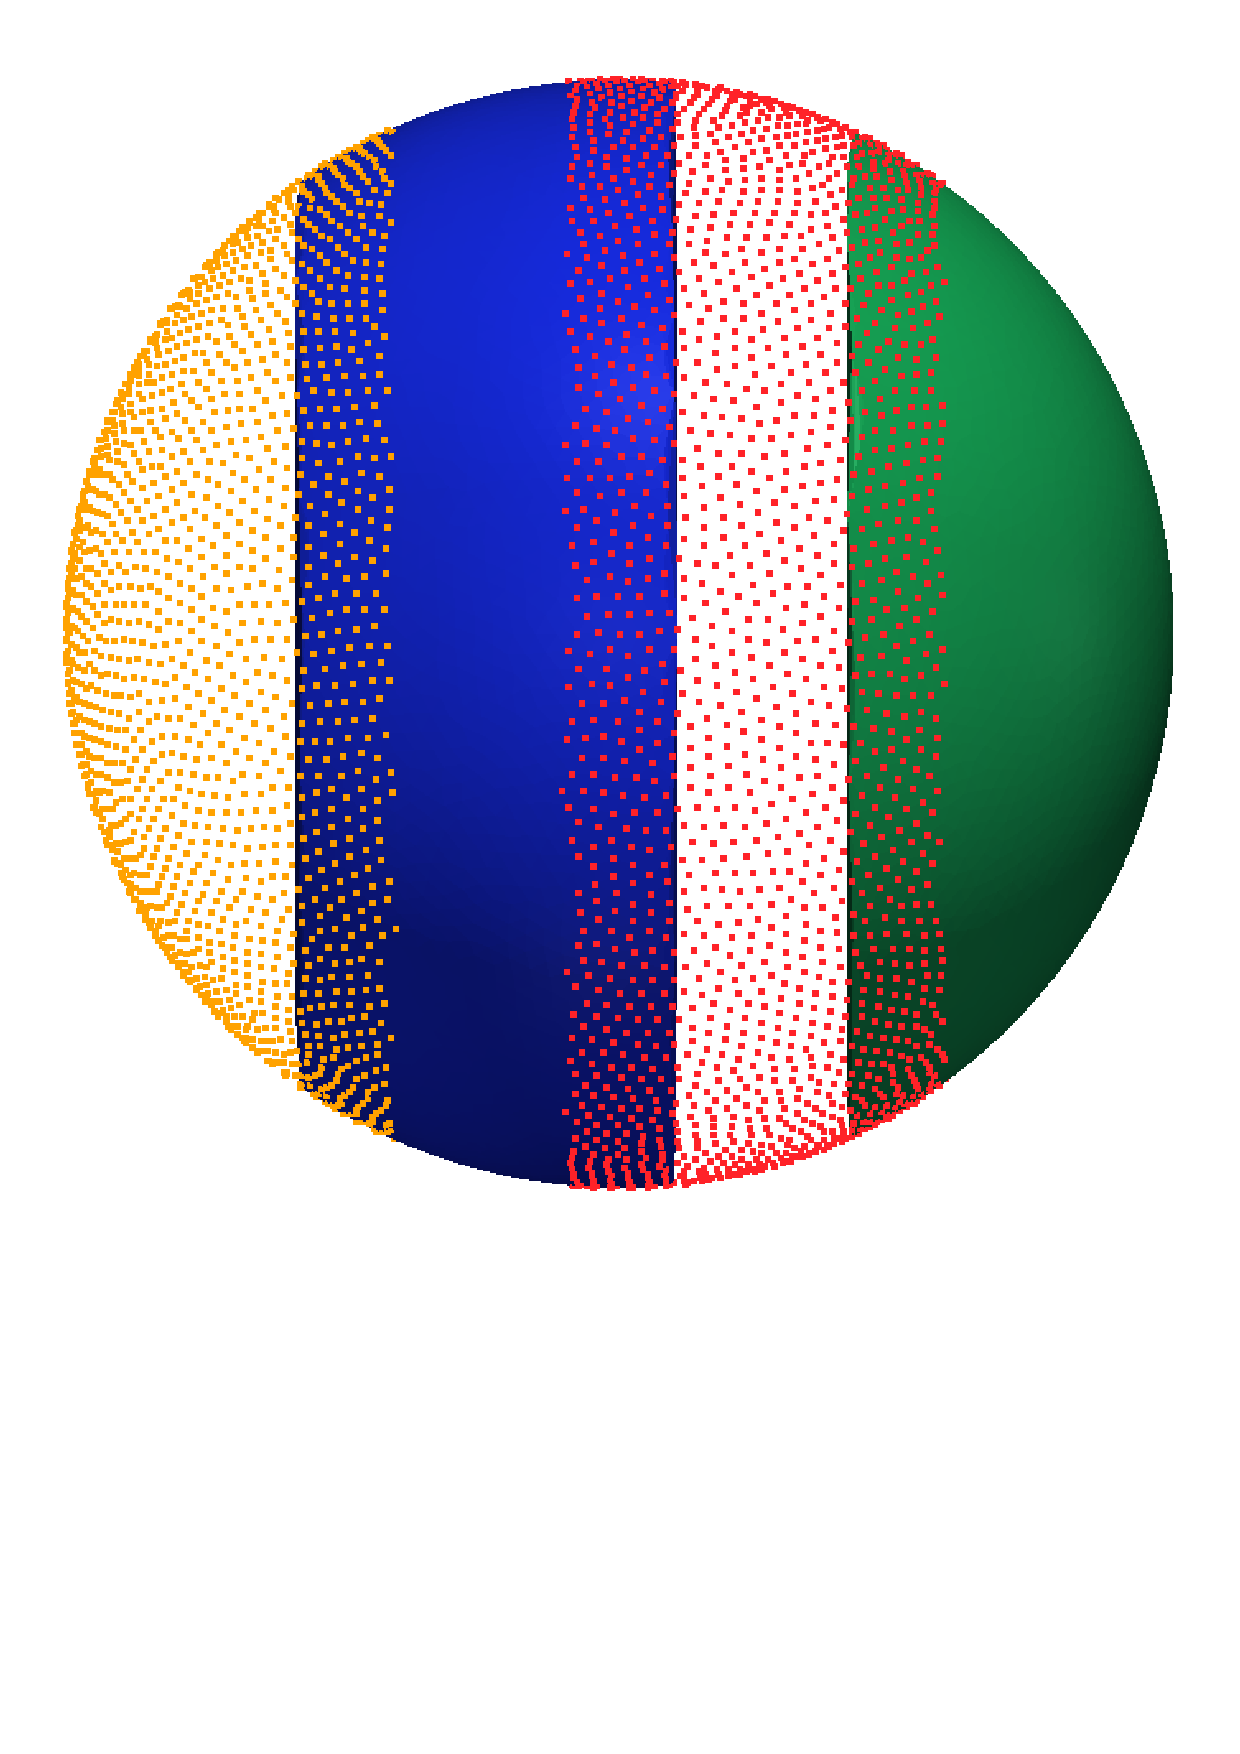
\includegraphics[width=2.5in]{../figures/paper1/figures/vortex_rollup/4procs_N10K_n31.pdf}
\caption{Partitioning of $N=10,201$ nodes to span four processors with stencil size $n=31$. }
\label{fig:decomposed_sphere}
\end{center}
\end{figure}

Linear partitioning is simple and easy to code. Each MPI process has at most two neighbors (left and right), so communication is straightforward. There are two concerns with this approach: 
\begin{enumerate} 
\item Scaling the number of processors can result in stencils spanning more than one narrow partitions in each direction. This introduces the need for complex communication collectives that go beyond just passing left and/or right.
\item In the case of irregular geometries, the partitioning of near uniform node distributions may result in imbalanced subdomains with unequal number of stencils.
\end{enumerate}

Alternative sphere partitionings exist. In atmospheric and geophysical communities for example, one often finds the cubed-sphere \cite{Ivan2011, Katta2012}, which transcribes a subdivided cube onto the sphere, and assigns projected rectangular subdivisions to individual processors. Another option is the icosahedral geodesic grid \cite{Randall2002}, which evenly balances the computational load by distributing equal sized geodesic triangles across processors. A complete list of options for partitioning the sphere is outside the scope of this work. %, but many involve recursive subdivisions based on simple geometric elements (i.e., triangle, rectangle, hexagon, etc.). 


\subsection{Graph Partitioning with METIS}

One of the major concerns when partitioning for a distributed environment is load balancing. Consider, for example, the situation where $p-1$ processors have equal sized partitions, each with $W_1$ amount of work, and a $p$-th processors is allocated some larger amount of work, $W_2$. In that case, the maximum possible speedup on $p$ processors obeys \cite{Gropp1990}:  
\begin{align}
S_p = \frac{(p-1) W_1 + W_2}{W_2} = 1 + (p-1)\frac{W_1}{W_2}.
\label{eq:load_balance}
\end{align}
The take-away from Equation~\ref{eq:load_balance} is that potential gains in parallelism are limited by the disproportionality of workloads. 

To ensure load balancing, one commonly turns to \emph{graph partitioning} algorithms. Formally, graph partitioning algorithms attempt to solve the $k$-way partitioning problem \cite{Karypis1999}: 

\begin{quote} Given a graph $G = (V,E)$ with vertices ($V$) and any number of edges ($E$), partition $V$ into $k$ subsets, $V_1, V_2, ..., V_k$ such that 
\begin{itemize} 
\item $V_i \cap V_j = \emptyset$ for $i \neq j$,
\item the size of each partition, $|V_i|$, is $|V_i| \approx \frac{N}{k}$, 
\item $\bigcup_i V_i = V$,
\item and the number of edges whose incident vertices belong to different $V_i$ is minimized.
\end{itemize}
\end{quote} 
In other words, we seek a partitioning that results in roughly equal sized subgraphs connected by as few edges as possible. 
In this case algorithms are applied to the adjacency graph produced by RBF-FD stencils (see \S~\ref{subsec:adjacency}).

The output from graph partitioning algorithms are ideal for distributed applications for two reasons. First, partitions of roughly equal size ensure a balanced workload across processors. Second, edges crossing partitions correspond to ghost node dependencies, so minimizing those connections also ensures minimized data transfer via MPI. 

A number of libraries exist for graph partitioning including Chaco \cite{CHACO1995}, SCOTCH \cite{SCOTCH1996}, and the METIS family of algorithms (e.g., METIS, ParMETIS, hMETIS) \cite{Karypis1999}. The algorithms vary by library, but in all cases vertex reordering and graph coloring capabilities are provided in addition to partitioning. %This work considers only the partitioning features.

Our latest work (in \cite{BolligRBFFDCode}) partitions graphs via METIS using the library's \emph{gpmetis} executable. During stencil generation, the associated adjacency graph is written to file. The METIS executable reads the file and performs a multi-level recursive bisection algorithm to partition the graph. At its core the algorithm first coarsens the graph into a sequence of smaller resolutions, applies a split to the smallest, and then pops back through the levels of recursion to project the coarse split onto finer graphs and smooth/correct the split at each level \cite{Karypis1999}. As input, METIS requires an undirected adjacency graph and the desired number of partitions. 
In return for the graph, METIS writes a file containing one integer per vertex, indicating the partition to which each stencil center is assigned. Note that METIS does not guarantee partitions will be contiguous. While this is often the case, METIS may find the alternative more fitting and assign disjoint subgraphs to the same MPI process. % for reduced communication. 

The adjacency graph for RBF-FD is directed, so symmetry is induced in the associated matrix with $A+A^T$. The added connectivity is harmless to RBF-FD as symmetry is only meant for partitioning purposes and does not impact actual DMs. With respect to load balancing: cutting an edge connecting a stencil center to a stencil node is equivalent to cutting its transpose. METIS is equally resistant apply a cut whether the edge is directed or undirected. 

\begin{figure}
\begin{center}
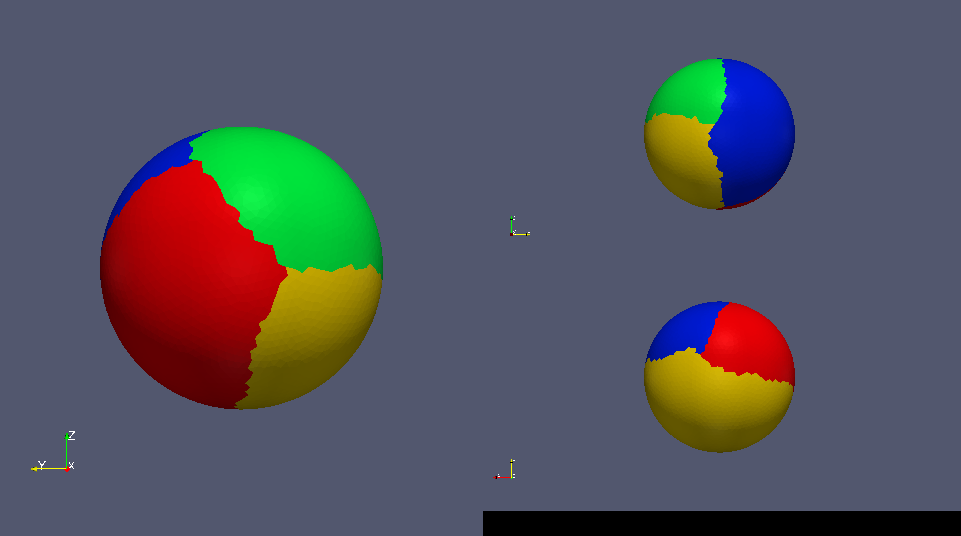
\includegraphics[width=0.8\textwidth]{rbffd_methods_content/decompositions/gpmetis_decomp_sphere_4parts.png}
\caption{METIS partitioning of $N=10,201$ nodes to span four processors with stencil size $n=31$. }
\label{fig:metis_decomposed_sphere}
\end{center}
\end{figure}

Figure~\ref{fig:metis_decomposed_sphere} provides an example of a METIS generated partitioning of $N=10,201$ MD nodes for four processors. Three camera angles show the sphere viewed from the $(-x)$-axis (left), $(+x)$-axis (top-right), and $(-z)$-axis (bottom-right). Overlap regions are not illustrated.

\subsection{A Load Balancing Comparison}
\label{sec:load_balance}

Table~\ref{tbl:load_balance} compares the load balance for linear and METIS-based partitionings of the unit sphere. The first two rows consider $p=4$ processes as shown in Figures~\ref{fig:decomposed_sphere} and \ref{fig:metis_decomposed_sphere}. Also shown in Table~\ref{tbl:load_balance} is the case of $p=16$ processors. 

We assume each partition has $N_p = N_i + N_r$ nodes where $N_i$ nodes are contained within each partition and $N_r$ are ghost nodes. Although values at the $N_r$ nodes are not computed within a partition, each process must still obtain their values. For the sake of argument we assume that the cost of communicating data for $N_r$ nodes is equivalent to the cost of computing them---in practice communication is much more expensive. Based on these assumptions, we consider the ratio of work across partitions, $\frac{W_1}{W_2} \approx \frac{\min N_p}{\max N_p}$, in the column labeled ``Total". Recall that ideal balancing is achieved at a ratio of 1. Columns labeled ``Interior" and ``Ghost Nodes" show the load balancing of only interior and overlap regions, respectively, in an effort to diagnose the source of imbalance across partitions. 

\begin{table}
\centering
\caption{Load balance comparison by partitioning for $N=10201$ MD-nodes on the unit sphere with stencil size $n=31$. A ratio of $1$ is ideal.}
\label{tbl:load_balance}
\begin{tabular}{c|c|c|c|c|c|c|c}
$p$ & Partitioning & Total ($\frac{\min N_p}{\max N_p}$) &  Interior ($\frac{\min N_i}{\max N_i}$) & Ghost Nodes ($\frac{\min N_r}{\max N_r}$)  \\ \hline
\multirow{2}{*}{4} & Linear  &  0.863 & 0.997 & 0.482  \\
& METIS  & 0.986 & 0.971 & 0.913   \\ \hline
\multirow{2}{*}{16} & Linear &  0.551 & 0.980 & 0.264   \\
& METIS & 0.925 & 0.942 & 0.864  \\
\end{tabular}
\end{table}
%\begin{table}
%\centering
%\caption{Load balance comparison by partitioning for $N=10201$ MD-nodes on the unit sphere with stencil size $n=31$. A ratio of $1$ is ideal.}
%\label{tbl:load_balance}
%\begin{tabular}{c|c|c|c|c|c|c|c}
%& $p$ & Total ($\frac{\min N_p}{\max N_p}$) &  Interior ($\frac{\min N_i}{\max N_i}$) & Ghost Nodes ($\frac{\min N_r}{\max N_r}$) & $\max(\frac{N_r}{N_p}) * 100\%$ \\ \hline
%\multirow{2}{*}{4} & Linear & 0.863 & 0.997 & 0.482 & 26.7\% \\
%& METIS & 0.986 & 0.971 & 0.913 & 16.7\% \\ \hline
%\multirow{2}{*}{16} & Linear & 0.551 & 0.980 & 0.264 & 61.1\% \\
%& METIS & 0.925 & 0.942 & 0.864 & 33.2\% \\
%\end{tabular}
%\end{table}
%
Based on the per process $N_p$'s, we find that linear partitioning works moderately well for $p=4$ but becomes horribly imbalanced at $p=16$. In both cases METIS proves significantly better with ratios $> 0.9$. Based on Table~\ref{tbl:load_balance} and Equation~\ref{eq:load_balance}, use of the linear partitioning should expect less than 9.3x speedup for $p=16$ processes, while METIS is bounded by at most 14.9x. Data for the partition interiors reveals that both linear and METIS partitioning distribute roughly equivalent number of nodes per interior---in fact, linear partitioning appears to be the more consistent of the two options. However, the problem with linear partitioning boils down to balancing ghost nodes. There are two obvious issues with linear partitioning:
\begin{itemize} 
\item End-cap partitions only have dependencies in on direction, whereas interior partitions have left and right dependencies. This immediately drops the ratio of $\frac{\min N_r}{\max N_r} \leq 0.5$. 
\item Since each overlap region is a small circle of the sphere and approximately $\sqrt{n}$ ghost nodes thick, the number of nodes in each region is therefore a function of its circumference. As $p$ grows $\frac{\min N_r}{\max N_r}$ scales as the ratio of the smallest and largest overlap region circumferences. 
\end{itemize}
While useful for development and testing, the conclusion is that even at moderate $p$ the situation is dire for linear partitions. METIS is preferred for consistent partition sizes and minimized overlap, but cautiously note the increasing imbalance in ghost nodes for METIS. Scaling tests in \S~\ref{sec:cpu_scaling} demonstrate that even METIS fails to find a partitioning of the graph that properly balances ghost nodes when $p$ is large.  

%DATA: 
%           G & R & O & Q
% Linear (4x): 3001/3479 & 448/928 & 425/952 & 2545/2553 & 928/3473
% METIS (4x): 3021/3064 & 461/505 & 442/483 & 2528/2603 & 505/3021
% Linear (16x): 901/1635 & 263/996 & 223/644 & 631/644 
% METIS (16x): 893/965 & 272/315 & 228/271 & 618/656
% 


\section{Index Mappings}

Once a partitioning is available, each MPI process is responsible for its own subset of nodes. 
To simplify accounting, we track nodes in two ways. Each node is assigned
a global index that uniquely identifies it. This index follows the node 
and its associated data as it is shuffled between processors. In addition, 
it is important to treat the nodes on each CPU/GPU in an identical manner. 
Implementations on the GPU are more efficient when node indices
are sequential. Therefore, we also assign a local index for the nodes on 
a given MPI process, which run from 1 to the maximum number of nodes on that process. 


It is convenient to break up the nodes on a given CPU into various sets
according to whether they are sent to other processors, are retrieved from 
other processors, are permanently on the processor, etc. Note as well, 
that each node has a home processor since the RBF nodes are partitioned into 
multiple domains without overlap.
Table~\ref{tbl:stencil_sets}, defines the collection of index lists that each CPU must maintain for both multi-CPU and multi-GPU implementations.  

        \begin{table}[t]
            \begin{center}
                \begin{tabular}{l l}
                    \hline
                    $\setAllNodes$ &: all nodes received and contained on the CPU/GPU $g$ \\
                    $\setCenters$ &: stencil centers managed by $g$ 
					(equivalently, stencils computed by $g$) \\
                    $\setBoundary$ &: stencil centers managed by $g$ that
                    require nodes from another CPU/GPU \\
                    $\setProvide$ &: nodes managed by $g$ that are sent to other CPUs/GPUs  \\
                    $\setDepend$ &: nodes required by $g$ that are managed by another CPU/GPU \\
                    \hline
                \end{tabular}
                \caption{Sets defined for stencil distribution to multiple CPUs}
                            \label{tbl:stencil_sets}
            \end{center}
        \end{table}
        
                \begin{figure}[ht] 
            \centering
            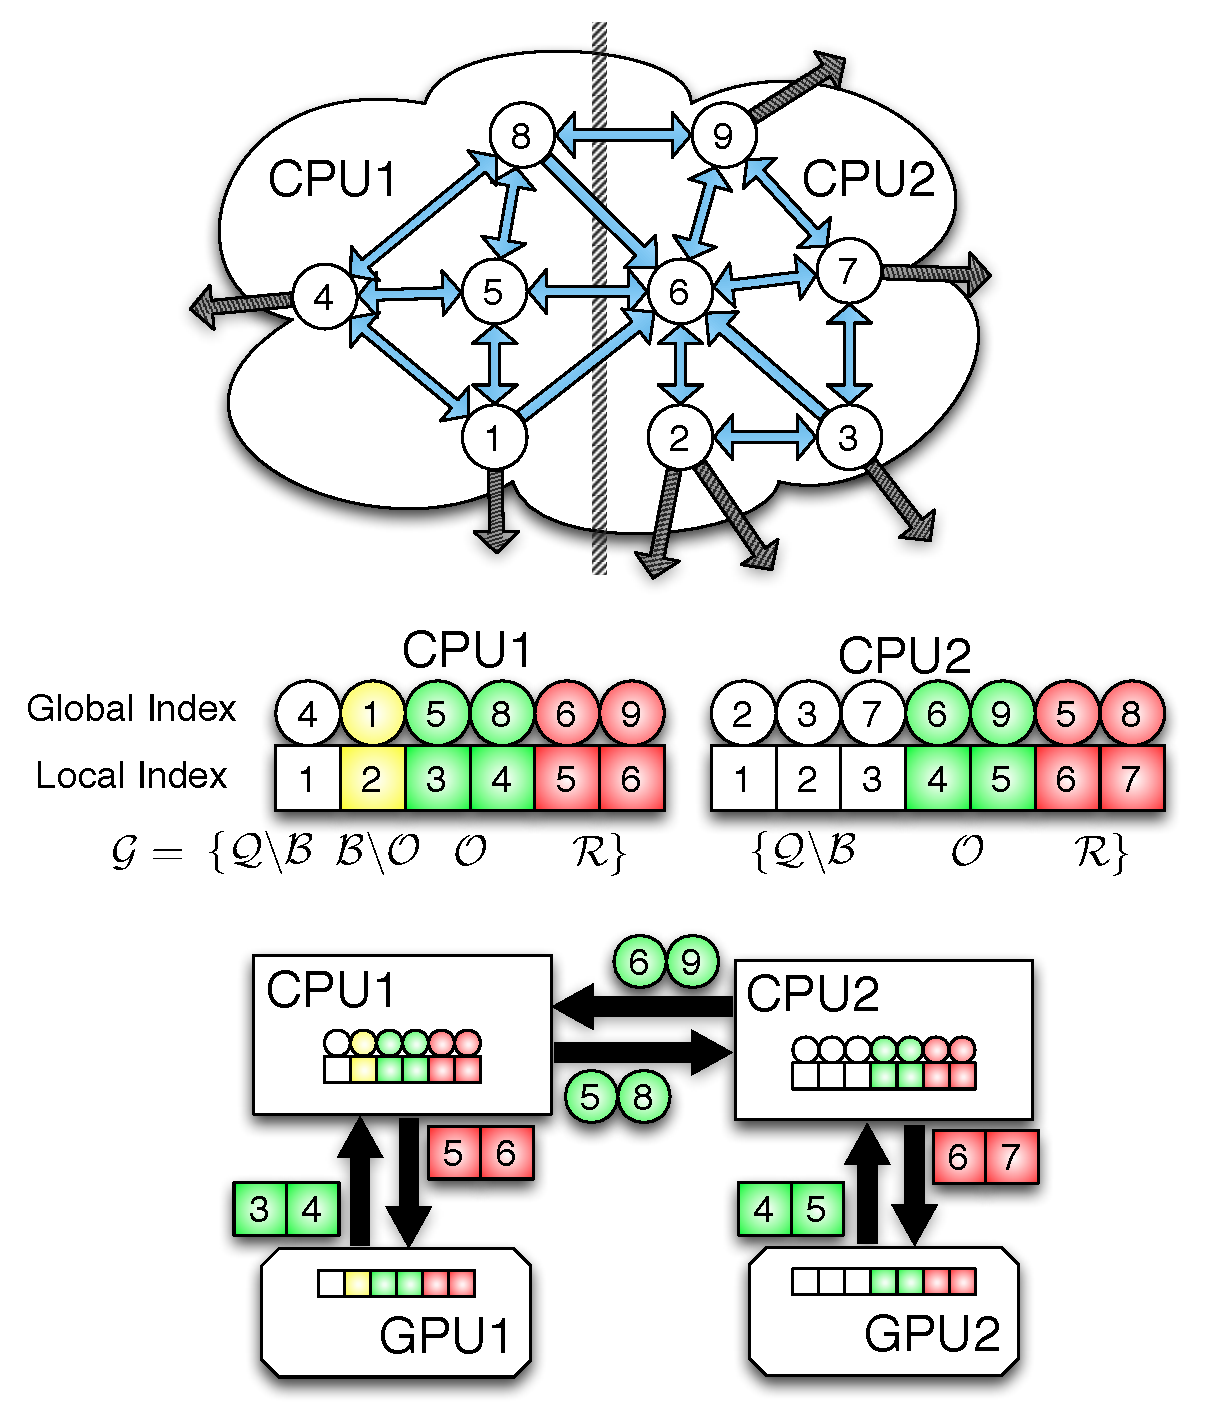
\includegraphics[width=3.5in]{../figures/paper1/figures/omnigraffle/SimpleExample.pdf} 
            \caption{Partitioning, index mappings and memory transfers for nine stencils ($n=5$) spanning two CPUs and two GPUs. Top: the directed graph created by stencil edges is partitioned for two CPUs. Middle: the partitioned stencil centers are reordered locally by each CPU to keep values sent to/received from other CPUs contiguous in memory. Bottom: to synchronize GPUs, CPUs must act as intermediaries for communication and global to local index translation. Middle and Bottom: color coding on indices indicates membership in sets from Table~\ref{tbl:stencil_sets}: $\setCenters \backslash \setBoundary$ is white, $\setBoundary \backslash \setProvide$ is yellow, $\setProvide$ is green and $\setDepend$ is red.
            }
            \label{fig:stencilSets2CPU}
        \end{figure}	

Refer to Figure~\ref{fig:stencilSets2CPU}, which illustrates a configuration with two 
CPUs and two GPUs, and 9 stencils, four on CPU1, and five on CPU2, separated
by a vertical line in the figure. Each stencil
has size $n=5$. At the top of Figure~\ref{fig:stencilSets2CPU}, stencils are laid out
with blue arrows pointing to stencil neighbors and creating the edges of the directed adjacency graph. Note that the connections between nodes are not 
always bidirectional. For example, node 6 is in the stencil of node 3, but 
node 3 is excluded from the stencil around 6. 
Gray arrows point to stencil neighbors outside the small window and are irrelevant in the following discussion focused only on data flow between two processes on CPU1 and CPU2. 
Since each process is responsible for the derivative evaluation and solution updates for any stencil center, it is clear that edges intersecting the vertical line point to ghost node dependencies. For example, node 8 on CPU1 has a stencil comprised of
nodes 4,5,6,9, and itself. The data associated with node 6 must be retrieved
from CPU2. Similarly, the data from node 5 must be sent to CPU2 to 
complete calculations at the center of node 6.
        
        
       
The center of Figure~\ref{fig:stencilSets2CPU} assigns the nine nodes to local sets for each process. The set of all nodes that a process interacts with is denoted by $\setAllNodes$, which includes both the stencil centers within the partition ($\Interior_i$), and all ghost nodes required to complete the calculations: $\bigcup_{j} \Gamma_{ij}$.  
We let $\setCenters\in\setAllNodes$ contain indices for all nodes within the partition $\Interior_i$. 
Then the set $\setDepend = \setAllNodes \backslash \setCenters$ contains indices of all ghost nodes. 
The set $\setProvide\in\setCenters$ indexes nodes that are needed in other partitions (i.e., $\bigcup_j \Gamma_{ji}$). The set $\setBoundary\in\setCenters$ consists of nodes dependent on values from $\setDepend$. Note that $\setProvide$ and $\setBoundary$ overlap, but can differ in size due to lack of symmetry in the adjacency matrix. To capture the difference, set $\setBoundary \backslash \setProvide$ are nodes that depend on $\setDepend$ but are not sent to other processes, while $\setCenters \backslash \setBoundary$ are nodes that have no dependency on information from other processes.

%TODO: cleanup: 
Constructing these index mappings allows each process to ignore nodes/stencils outside their subdomain and focus only on their subset of the problem. Processes avoid both the cost of storing a complete RBF-FD differentiation matrix (DM) as well as full solution vectors. Instead, a local rectangular DM of size $|\setCenters| \times |\setAllNodes|$ is constructed by each process with compressed solution vectors of size $|\setAllNodes|$ to match. Our implementation follows a workflow that first generates stencils, and then partitions the adjacency graph in serial. In parallel, each processor loads its assigned partition, constructs index mappings, and solves for RBF-FD weights to generate a local DM.  

\section{Local Ordering}

Figure~\ref{fig:stencilSets2CPU} lists global node indices contained in $\setAllNodes$ for each MPI process. Global indices are paired with a local mapping to indicate the internal node ordering for each process. The structure of set $\setAllNodes$,
   \begin{equation}
 		\setAllNodes = \{ \mathcal{Q}\backslash\mathcal{B} \ \ \mathcal{B}\backslash\mathcal{O} \ \ \mathcal{O} \ \ \setDepend \},
            \label{eq:decompose_g}
        \end{equation}
 is designed to simplify both CPU-CPU and CPU-GPU memory transfers by grouping nodes of similar type. The color of the global and local indices in the figure
 indicate the sets to which they belong. They are as follows: white represents $\setCenters \backslash \setBoundary$, 
 yellow represents $\setBoundary \backslash \setProvide$, green indices 
 represent $\setProvide$, and red represent $\setDepend$.  


 The structure of $\setAllNodes$ offers two benefits: first, solution values in $\setDepend$ and $\setProvide$ are contiguous in memory and can be copied to or from the GPU without the filtering and/or re-ordering normally required in preparation for efficient data transfers. Second, asynchronous communication allows for the overlap with computation, where distinguishing the set $\mathcal{B}$ allows the computation of $\mathcal{Q}\backslash \mathcal{B}$ without waiting on MPI communication to send and receive $\mathcal{O}$ and $\mathcal{R}$. 

When targeting the GPU, communication of solution or intermediate values is a multi-step process:
   \begin{enumerate}
    \item Transfer $\mathcal{O}$ from GPU to CPU
    \item Encode $\mathcal{O}$ to send buffer
	\item Distribute $\mathcal{O}$ to other CPUs and receive $R$ from other CPUs
	\item Decode $\mathcal{R}$ from received buffer  
	\item Transfer $\mathcal{R}$ to the GPU
	\item Launch a GPU kernel to operate on $\mathcal{Q}$
   \end{enumerate} 
The data transfers involved in this process are illustrated at the bottom of Figure~\ref{fig:stencilSets2CPU}.
    Each GPU is only aware of the local indexing in Equation~\ref{eq:decompose_g}. Benefiting from the local structure, set 
$\setProvide$ is copied off the GPU and into CPU memory as one contiguous memory block. The CPU is then responsible for an \emph{encode} process that maps local to global indices, copies elements of $\setProvide$ into an MPI buffer with one entry for each receiving CPU (i.e., data is grouped by destination). MPI distributes the encoded buffer and receives $\setDepend$ in a buffer that is sorted by origin. In general, Equation~\ref{eq:decompose_g} need not have $\setDepend$ structured the same as the receive buffer (i.e., data grouped by origin process). However, if the two do not match then received data must go through a \emph{decode} process to shuffle elements into the proper local ordering. The reordered data is then copied as a contiguous block of memory to the GPU. Decoding data is avoided with a simple assumption on the ordering of $\setDepend$. In \S~\ref{sec:cpu_scaling} bypassing the decode phase is one of several strategies employed for improved scalability. 

\begin{figure}
\begin{center}
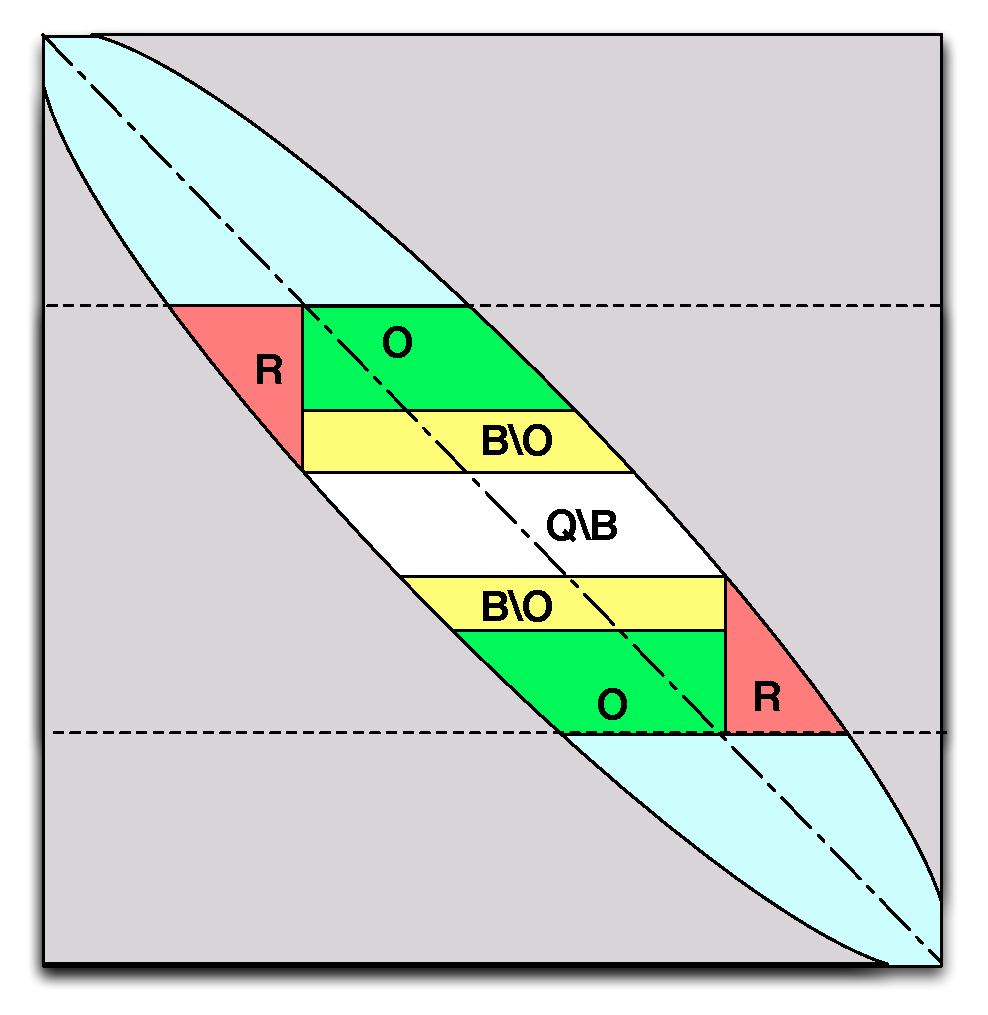
\includegraphics[width=0.45\textwidth]{rbffd_methods_content/decompositions/MatrixDecompositionSets_RBF-FD_Bowed.pdf} 
\caption{Decomposition for one processor selects a subset of rows from the DM. Blocks corresponding to node sets $\setCenters \backslash \setBoundary$, $\setProvide$, and $\setDepend$ are labeled for clarity. The subdomain/partition is outlined by dashed lines.}
\label{fig:decomp_matrix_view}
\end{center}
\end{figure}

\subsection{Local Differentiation Matrix (DM) Structure}

The local ordering of nodes leads to a unique DM on each MPI process. Consider Figure~\ref{fig:decomp_matrix_view} which shows the index sets for a single partition in context of a global RBF-FD differentiation matrix. Here the gray area is zero, and non-zeros exist between bowed lines. The partition is illustrated as the contiguous set of rows between dashed lines. Set membership for each row is determined based on how the off-diagonal non-zeros in a row match vertically with the center diagonal. When an MPI process constructs the local DM for the partition, the two sets of $\mathcal{B}$ in Figure~\ref{fig:decomp_matrix_view} are compressed into one contiguous set. %An example of this effect is demonstrated in Figure~\ref{fig:decomp_spy}. 

Figure~\ref{fig:decomp_spy} demonstrates the structure of a local DM on an MPI process. Labels denote the components of Equation~\ref{eq:decompose_g}. The local DM represents partition three of four from an original matrix with $N=4096$ rows and $n=31$ non-zeros per row. The RBF-FD stencils were generated on the $N=4096$ MD node set, and partitioned with METIS. 
\begin{figure}
\begin{center}
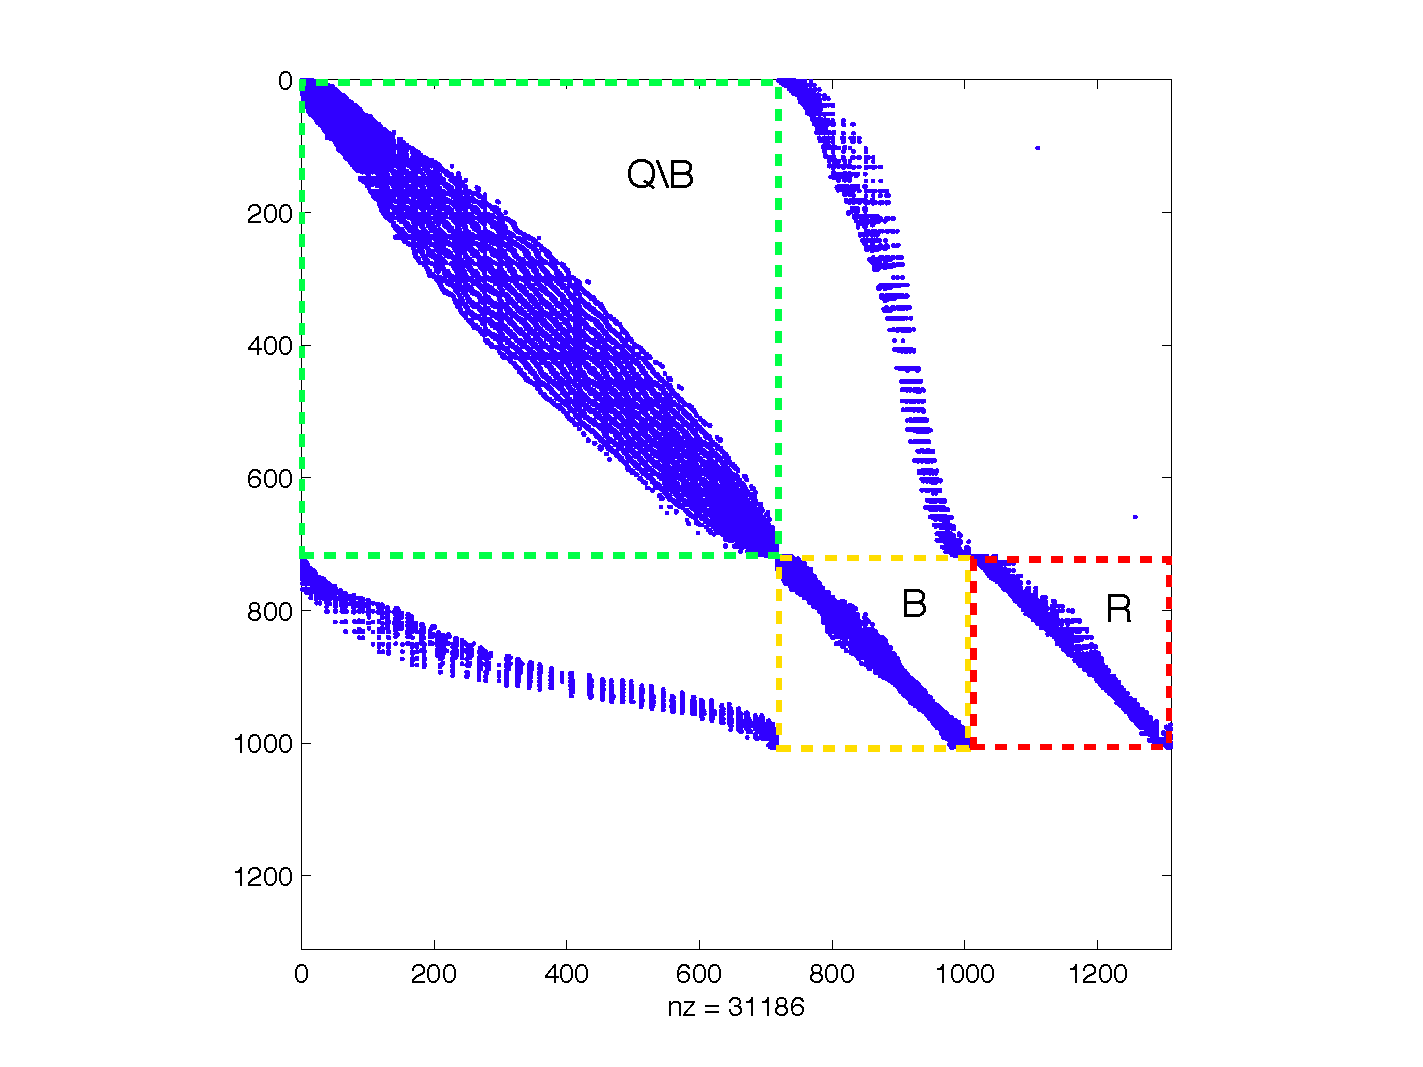
\includegraphics[width=9cm]{rbffd_methods_content/decompositions/spy_metis_stencil_example_labels.png}
%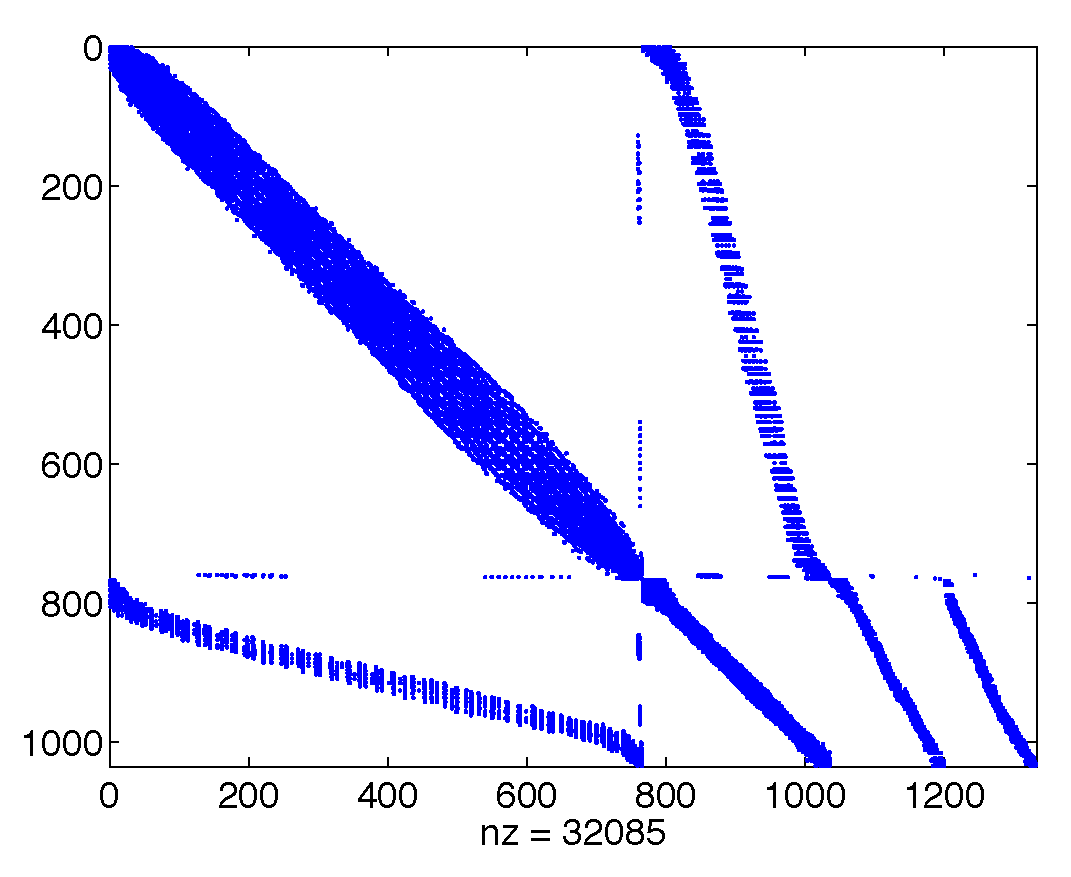
\includegraphics[width=0.45\textwidth]{rbffd_methods_content/decompositions/spy_metis_stencil_example_part_2_of_4.pdf}
\caption{Spy of the local DM on processor 3 of 4 from a METIS partitioning of $N=4096$ nodes with stencil size $n=31$ and stencils generated with Algorithm~\ref{alg:fixed_grid_query} ($hnx=100$). Blocks are highlighted to distinguish node sets $\setCenters \backslash \setBoundary$, $\setBoundary$, and $\setDepend$. $\setDepend$ Stencils involved in MPI communications have been permuted to the bottom of the matrix. The split in $\setDepend$ indicates communication with two neighboring partitions. }
\label{fig:decomp_spy}
\end{center}
\end{figure}



%TODO: Domain boundary nodes appear at beginning of the list 

\section{Communication Collectives}
\label{sec:mpi_collectives}

With a partitioning and local ordering decided, communication collectives are established to transfer data between MPI processes. Two types of collectives are possible: all-to-all and all-to-subset. 

All-to-all collectives pass data from every processor to all other processors. The most basic MPI implementation of an all-to-all, the MPI\_Alltoall routine, is illustrated in Figure~\ref{fig:mpi_alltoall_visual}. For a cluster of $p$ processes, MPI\_Alltoall assumes that every process intends to send $N_p$ bytes to all $p-1$ processors. On the left, an output buffer with $p*N_p$ bytes is assembled locally on each process. Block sizes in Figure~\ref{fig:mpi_alltoall_visual} are indicative of the number of bytes sent to each process. The subscripts on example data A, B, C indicate the destination process.  When the collective executes, MPI\_Alltoall scatters $N_p$ bytes from all processes to effectively interchange/transpose data on the right of Figure~\ref{fig:mpi_alltoall_visual}. 

\begin{figure}
\centering
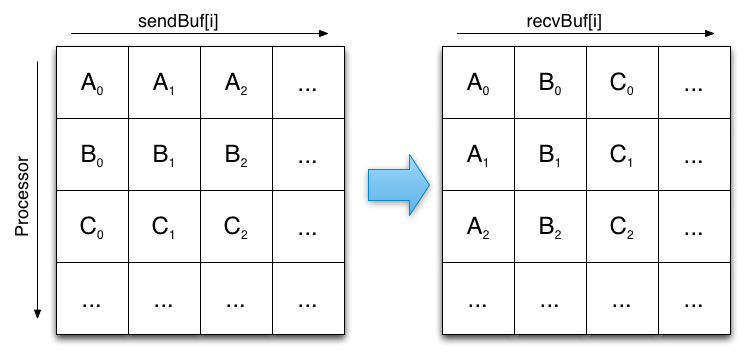
\includegraphics[width=10cm]{../figures/omnigraffle/MPI_Alltoall_Visual.png}
\caption{An ``all-to-all" communication collective interchanges/transposes data across processes. All processors (e.g., 0, 1, 2) connect and transmit data subsets (e.g., A, B, C) to every other processor.}
\label{fig:mpi_alltoall_visual}
\end{figure}

%All-to-all collectives are only useful when data needs to be simultaneously interchanged between all processes. 
Since RBF-FD partitioning via METIS restricts overlap to a subset of neighboring partitions, it makes sense to adopt an all-to-subset approach and avoid the overhead of unnecessary connections and memory padding required by MPI\_Alltoall. 
Two types of all-to-subset are illustrated in Figures~\ref{fig:mpi_alltoallv_visual} and \ref{fig:mpi_isendirecv_visual}. 


\begin{figure}
\centering
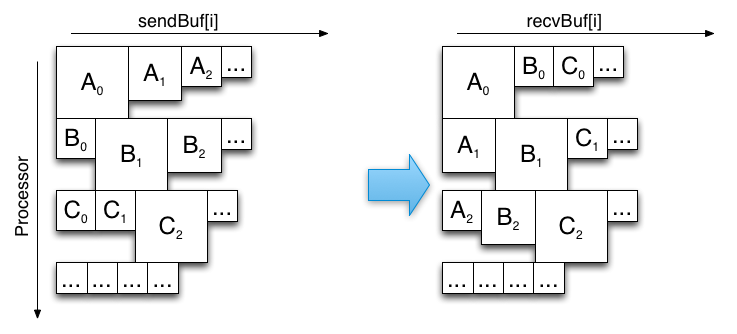
\includegraphics[width=10cm]{../figures/omnigraffle/MPI_Alltoallv_Visual.png}
\caption{RBF-FD interchanges a variable number bytes between processes. An ``all-to-subset" collective implemented via the MPI\_Alltoallv collective compresses the interchange by allowing variable message sizes between processors. Zero-byte connections are skipped by the routine internally.}
\label{fig:mpi_alltoallv_visual}
\end{figure}

Figure~\ref{fig:mpi_alltoallv_visual} shows the behavior of an MPI\_Alltoallv. MPI\_Alltoallv improves on the all-to-all counterpart by allowing variable message sizes per connection. Unpadded messages transmit fewer bytes and reduce the overall communication time. Implementations of MPI\_Alltoallv detect \emph{zero-byte messages} (i.e., empty messages), and skip connections to their intended processes. This gives the routine an all-to-subset behavior. Note that MPI\_Alltoallv should be used with caution: while zero-byte connections are avoided, the overhead in checking message sizes grows with the number of processors. For very large $p$ the communication time can be dominated by those operations, defeating the gains in all-to-subset connection (see e.g., \cite{Balaji2010}). 


%TODO: 
% cost of communciation is high 
% amdahls law states that we are limited by the serializable portion of 
% so we want to hide it as much as possible
%

MPI\_Alltoallv is also a blocking collective: when the routine is called, all communication must complete before control is returned to computation. This blocking behavior prevents the use of MPI\_Alltoallv in overlapping communication and computation within a distributed CPU environment. A distributed GPU environment can overlap MPI\_Alltoallv communication due to the non-blocking behavior of GPU commands (this is tested in Chapter~\ref{chap:multigpu_rbffd}). As of this writing, a new version of the MPI standard (v3.0) introduces MPI\_Ialltoallv, a non-blocking collective that would allow overlap on the CPU \cite{MPI}. MPI\_Ialltoallv is not considered here as popular MPI distributions did not yet offer MPI v3.0 compliant implementations.

\begin{figure}
\centering
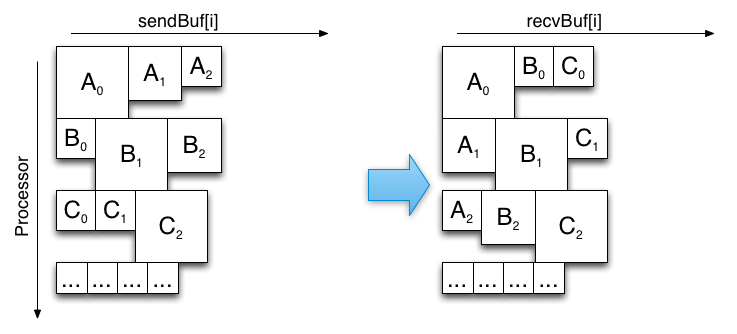
\includegraphics[width=10cm]{../figures/omnigraffle/MPI_IsendIrecv_Visual.png}
\caption{A true ``all-to-subset" collective based on direct sends and receives allows for variable message sizes, and strictly truncates the number of connections between processors to only required connections. This collective is implemented with MPI\_Send/MPI\_Recv or MPI\_Isend/MPI\_Irecv.}
\label{fig:mpi_isendirecv_visual}
\end{figure}

Figure~\ref{fig:mpi_isendirecv_visual} shows a true all-to-subset collective implemented with direct sends and receives between processes that are either blocking (MPI\_Send, MPI\_Recv) or non-blocking (MPI\_Isend, MPI\_Irecv). Processes strictly communicate with required neighbors, so no zero-byte messages inflate communication time. 
A blocking version of this all-to-subset was employed in our first paper (\cite{BolligFlyerErlebacher2012}) for debugging purposes. MPI sends and receives were issued in a round-robin fashion. Unfortunately, the serialized connections made it infeasible to target $p > 10$. 

In an effort to improve performance and scaling of our implementation an MPI\_Alltoallv was employed. Appendix~\ref{app:keeneland_alltoallv_benchmarks} presents benchmarks of the improved collective running on Keeneland for comparison with our first paper. Appendix~\ref{app:spear_alltoallv_benchmarks} benchmarks the MPI\_Alltoallv collective on the FSU Spear cluster. Both appendices consider the scaling of the distributed SpMV on a small number of nodes.  

In what follows the MPI\_Alltoallv implementation is taken as baseline for communication. An attempt is then made to further reduce communication times and improve the scaling of our implementation in a distributed CPU environment. By focusing on the CPU-only environment we can test scaling on moderately large $p$ (we go up to $p = 1024$). Scaling improvements for the CPU-only environment similarly improve the distributed GPU implementation (see Chapter~\ref{chap:multigpu_rbffd}). 

\section{Scaling Improvements} 
\label{sec:cpu_scaling}


Two types of scaling are considered: weak and strong. Weak scaling monitors the growth in run-time as the number of processes ($p$) increases with the a constant workload per process, $N_p$. In other words the global problem size grows as $N = p*N_p$. Strong scaling keeps a fixed global problem size to consider $N_p = \frac{N}{p}$, where processes are issued diminishing workloads as $p$ grows. 
The scalings reveal different properties:
\begin{itemize} 
\item Weak scaling demonstrates the ability run problem sizes that are too large for a single CPU. Ideal weak scaling implies that the total run-time remains constant as additional parallelism is added. %Growth in run-time under weak-scaling most can problems with communication and ghost node load imbalances. 
\item Strong scaling finds the point at which the cost of communication overcomes the cost of computation. Ideal strong scaling is linear in terms of speedup (i.e., $S_p = p$), but to achieve it is unrealistic due to the serial cost of communication. 
\end{itemize}
 

For both scalings a simple idealized problem is tested where four derivatives are computed over a regular grid in 3-D and used as the intermediate vectors for an RK4 time-step. At the end of each SpMV a communication collective synchronizes the local derivative vectors. At the end of one thousand iterations, each process computes the local norm of the latest vector and an MPI\_Reduce collects global norms for verification. Timings are reported for the distributed SpMV including MPI communication using \emph{gettimeofday}.

Stencil sizes $n=17, 31, 50$ and $101$ are tested. Weak scaling is evaluated for $N_p=4000$ per processor. Strong scaling considers $N=4096000$ (i.e., $N=160^3$) nodes. Timings are reported for total execution time in a distributed SpMV, as well as per-component times for computation and communication only.


Verification details are not reported here since they are only significant in ensuring that parallel results are consistent. 


The benchmark is run on the Itasca HPC cluster at the University of Minnesota (Minnesota Supercomputing Institute). Itasca has 1,134HP ProLiant blade servers, each with two-socket, quad-core 2.8 GHz Intel Xeon processors. Each compute node has at least 24GB of RAM. Itasca has a total of 8,744 cores available for computing with a total usable memory size of 31.3 TB \cite{MSIItasca}. Test cases are compiled with the Intel v2013.5 compiler (``icc") and the Intel provided MPI (``IMPI"). Optimization flag ``-O3" is used to enable auto-vectorization, loop unrolling, blocking, etc.

Itasca's InfiniBand network topology is a 2-way fat-tree network. Each compute node, with 8 cores, is considered a \emph{leaf} of the fat-tree. Processes within a leaf communicate via shared memory. Groups of 16 nodes connect via QDR InfiniBand to \emph{leaf switches} at the second level of the tree. All leaf switches are in turn connected to two director nodes via 4x QDR InfiniBand. The topology exhibits 8:1 contention between nodes of the same leaf and additional 2:1 contention between leaf switches \cite{ItascaTuning}. Our implementation of RBF-FD does not detect or adjust to network topology, so network contention may inflate communication times. Tuning for the network topology is reserved for future work. 



\subsection{Baseline: MPI\_Alltoallv}

As a baseline for discussion, consider Figure~\ref{fig:strong_scaling_alltoallv} which shows the strong scaling achieved on Itasca with an MPI\_Alltoallv collective. Strong scaling is assessed in terms of speedup: $S_p = \ ^{t_1}/_{t_p}$ where $t_1$ is the serial time and $t_p$ is parallel time. The average execution times for the distributed SpMV are provided in Figure~\ref{fig:strong_scaling_alltoallv_all_stencils} with corresponding speedups relative to the single process execution in Figure~\ref{fig:strong_scaling_speedup_alltoallv_all_stencils}. For $p <= 8$ the scaling is poor due to the growing number of processes on the same compute node contending for shared memory. The code scales well (i.e., nearly linear) between 8 and 128 processes, but the gains taper off beyond $p > 128$. Per-component data for the MPI\_Alltoallv test case reveals the expected linear decrease in computation for $p>8$ (see Figure~\ref{fig:strong_scaling_spmv_only_alltoallv_all_stencils}), and eventually the communication time exceeding computation time at $p \geq 128$ (see Figure~\ref{fig:strong_scaling_comm_only_alltoallv_all_stencils}). 


\begin{figure} 
\centering
\begin{subfigure}{0.48\textwidth}
\centering
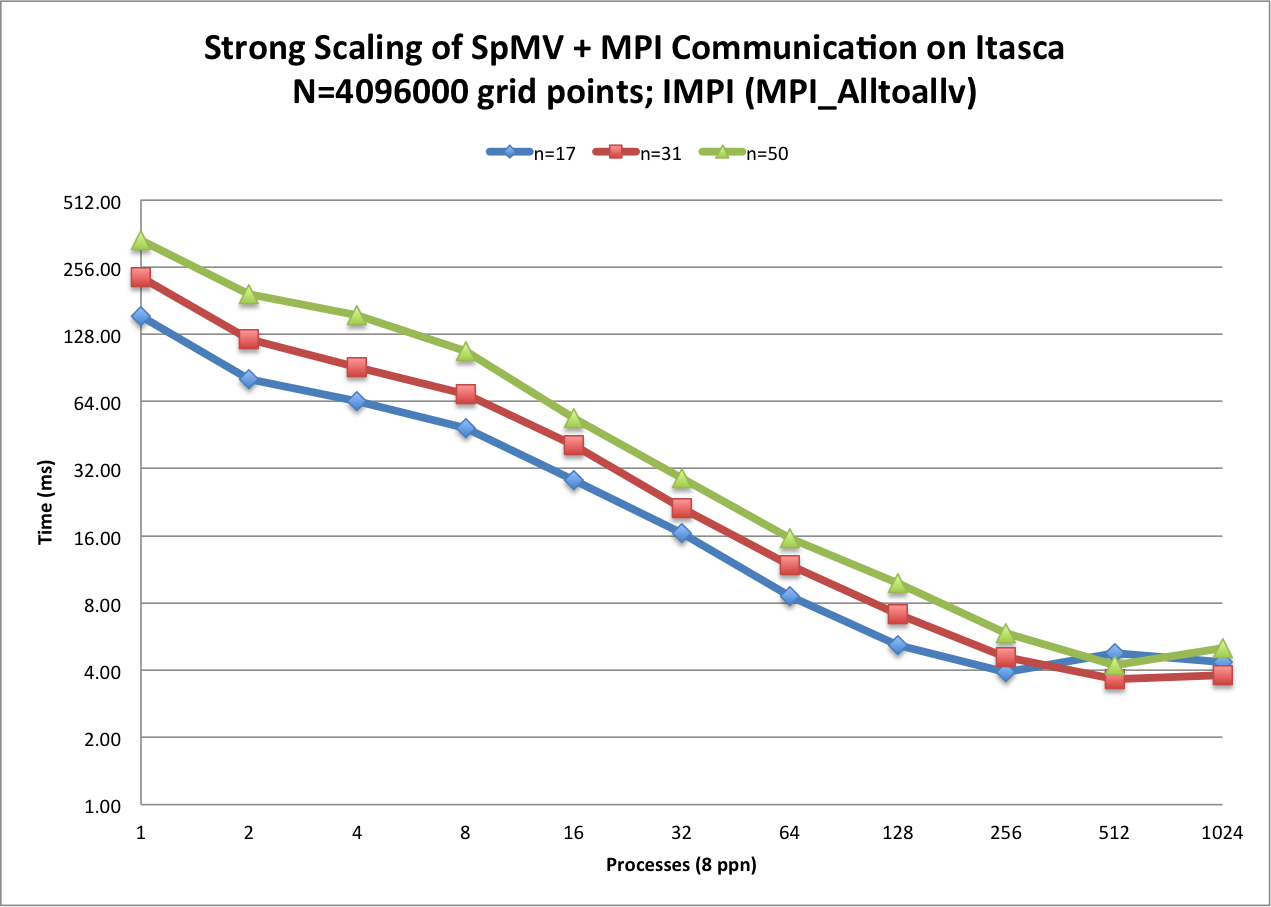
\includegraphics[width=\textwidth]{performance_content/scaling/strong_scaling_4M_regular_alltoallv.png}  
\caption{Strong scaling}
\label{fig:strong_scaling_alltoallv_all_stencils}
\end{subfigure}
\begin{subfigure}{0.48\textwidth}
\centering
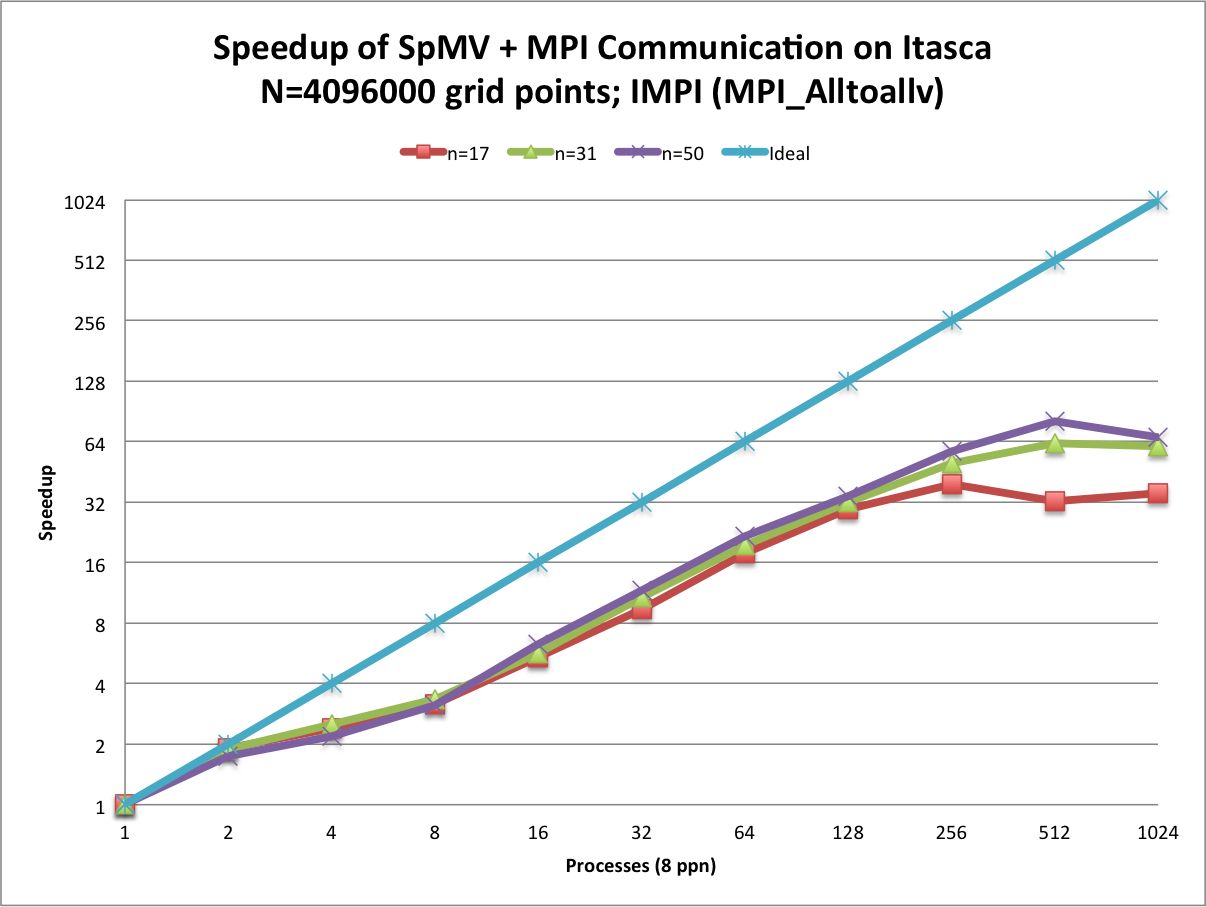
\includegraphics[width=\textwidth]{performance_content/scaling/strong_scaling_4M_regular_alltoallv_speedup.png}
\caption{Speedup ($S_p = \ ^{t_{1}}/_{t_p}$)}
\label{fig:strong_scaling_speedup_alltoallv_all_stencils}
\end{subfigure}
\caption{Strong scaling of the distributed SpMV on $N=4096000$ nodes (i.e., a $160^3$ regular grid) and various stencil sizes. Communication handled by MPI\_Alltoallv. }
\label{fig:strong_scaling_alltoallv}
\end{figure}

\begin{figure} 
\centering
\begin{subfigure}{0.48\textwidth}
\centering
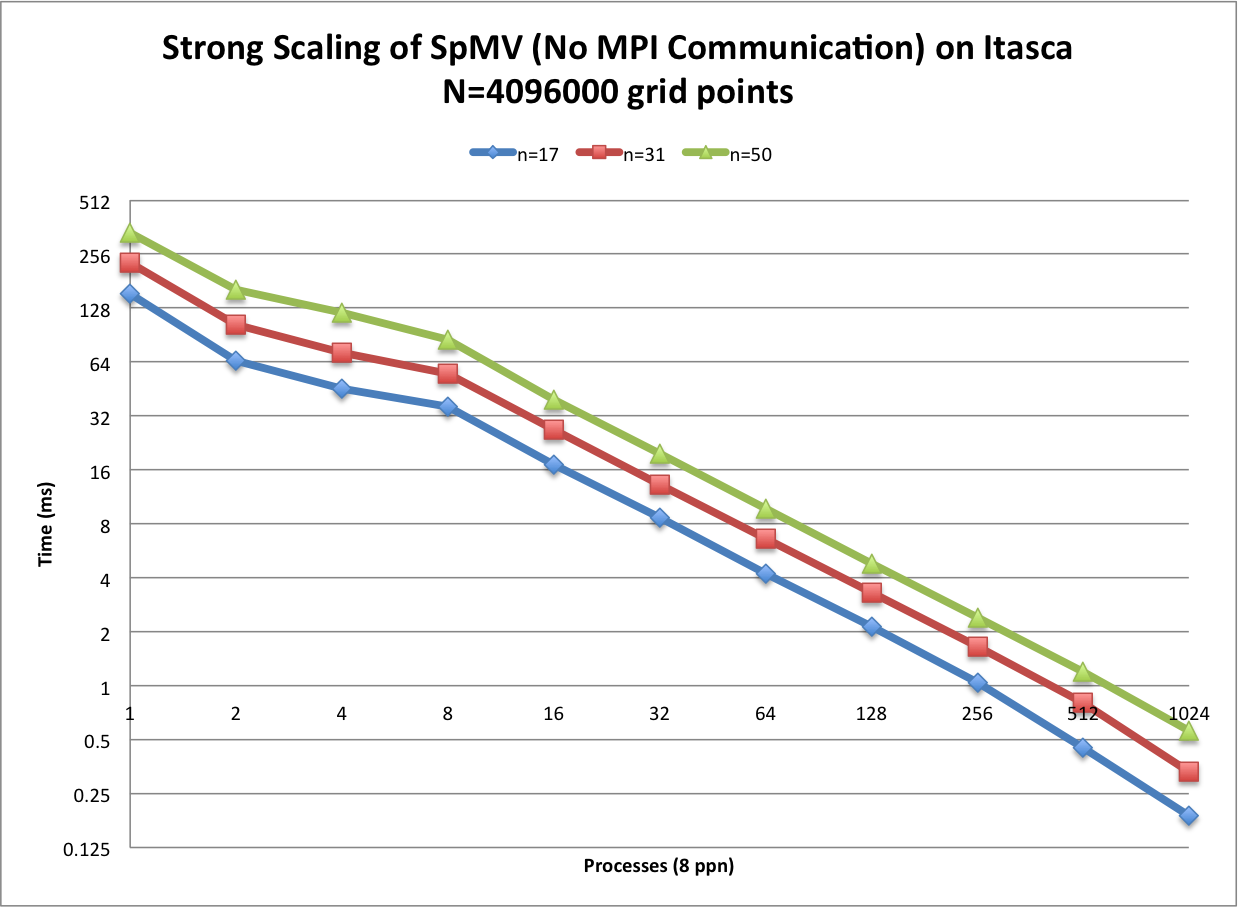
\includegraphics[width=\textwidth]{performance_content/scaling/strong_scaling_4M_regular_spmvOnly.png}
\caption{SpMV only}
\label{fig:strong_scaling_spmv_only_alltoallv_all_stencils}
\end{subfigure}
\begin{subfigure}{0.48\textwidth}
\centering
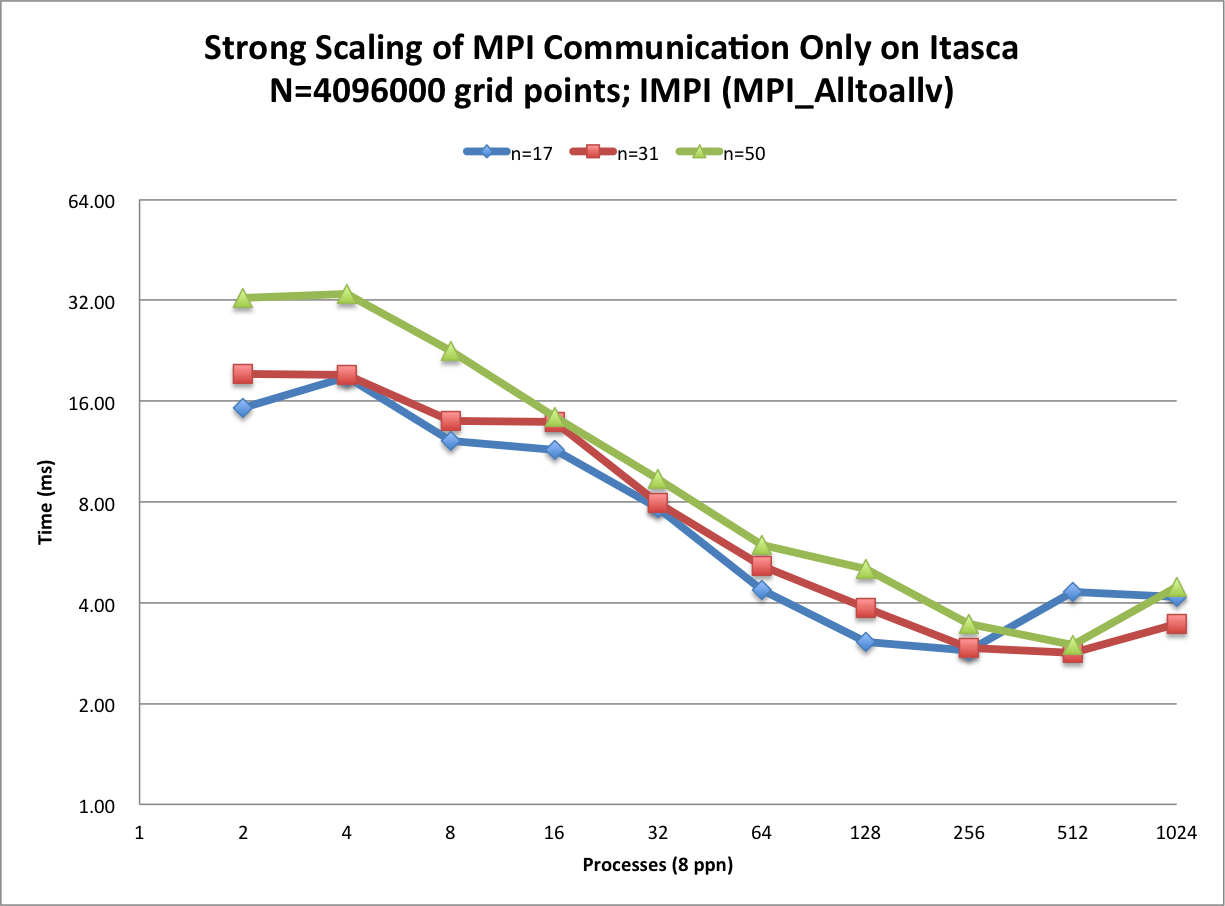
\includegraphics[width=\textwidth]{performance_content/scaling/strong_scaling_4M_regular_alltoallv_commOnly.png} \caption{Communication Only (MPI\_Alltoallv)}
\label{fig:strong_scaling_comm_only_alltoallv_all_stencils}
\end{subfigure}
\caption{Per-component benchmarks for strong scaling benchmarks on $N=4096000$ nodes. Communication time outweighs computation time for $p>128$ processes.  }
\label{fig:per_component_strong_scaling_alltoallv}
\end{figure}


The data in Figure~\ref{fig:weak_scaling_comm_only_alltoallv_all_stencils} shows MPI\_Alltoallv weak scaling is poor. As $p$ grows, the total time follows at a discouraging rate. Figure~\ref{fig:weak_scaling_spmv_only_alltoallv_all_stencils}, which presents the SpMV (computation) time only, verifies that beyond the initial contention on a single compute node, the SpMV is constant for all stencil sizes. That then implies the cost of communication could be reduced (or hidden). 

\begin{figure}
\centering
\begin{subfigure}{0.48\textwidth}
\centering
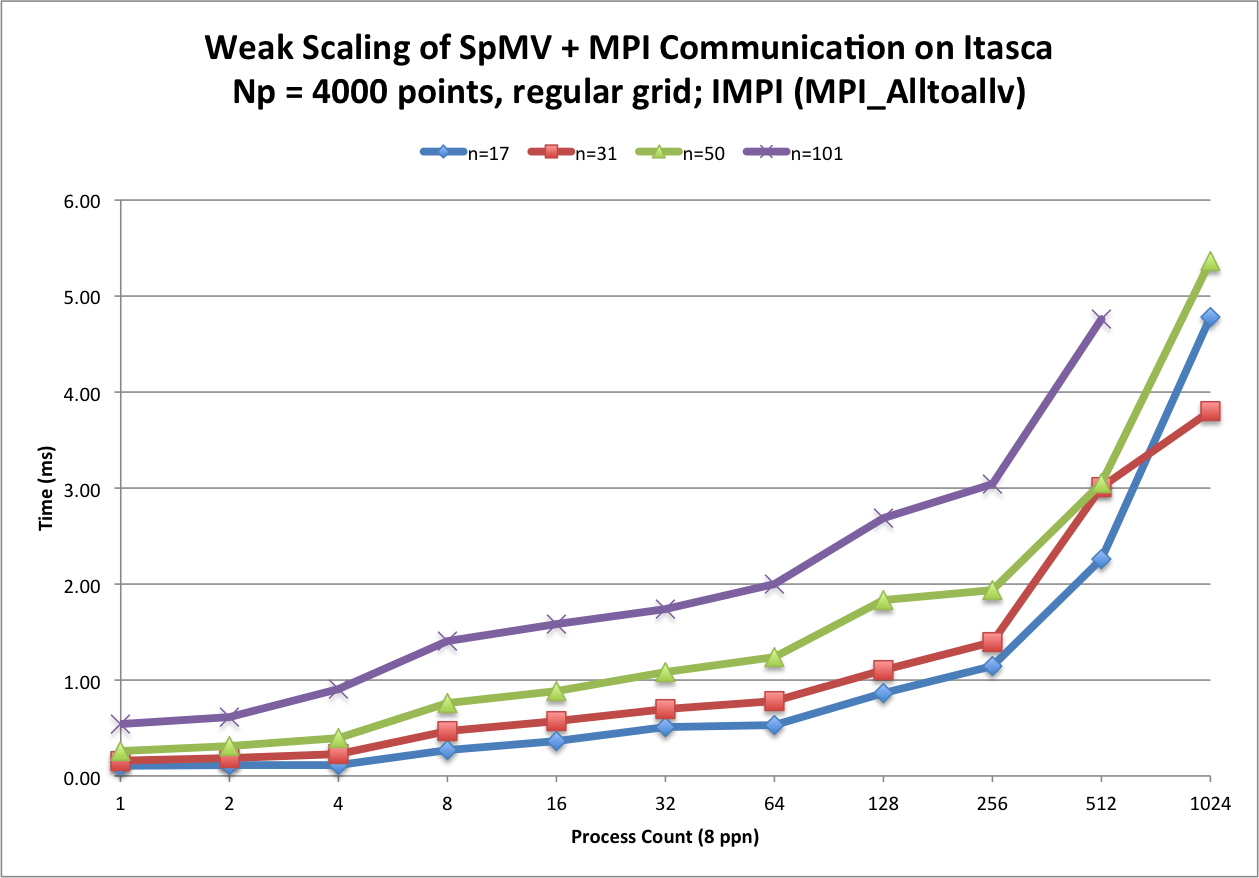
\includegraphics[width=\textwidth]{performance_content/scaling/weak_scaling_np4000_regular_alltoallv.png}\caption{Weak Scaling}
\label{fig:weak_scaling_comm_only_alltoallv_all_stencils}
\end{subfigure}
%\begin{subfigure}{0.48\textwidth}
%\centering
%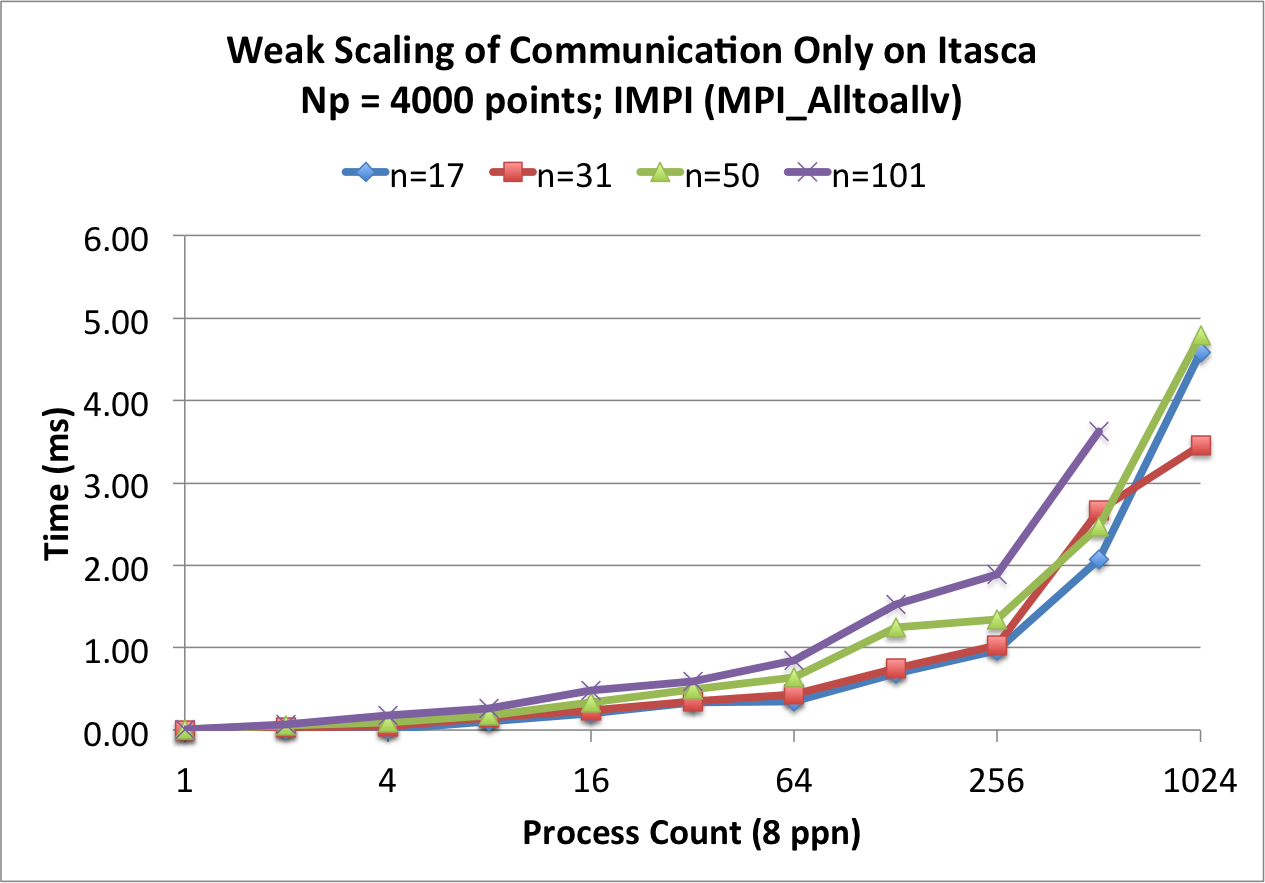
\includegraphics[width=\textwidth]{performance_content/scaling/weak_scaling_np4000_regular_alltoallv_commOnly.png}
%\caption{MPI\_Alltoallv only}
%\label{fig:weak_scaling_comm_only_alltoallv_all_stencils}
%\end{subfigure}
\begin{subfigure}{0.48\textwidth}
\centering
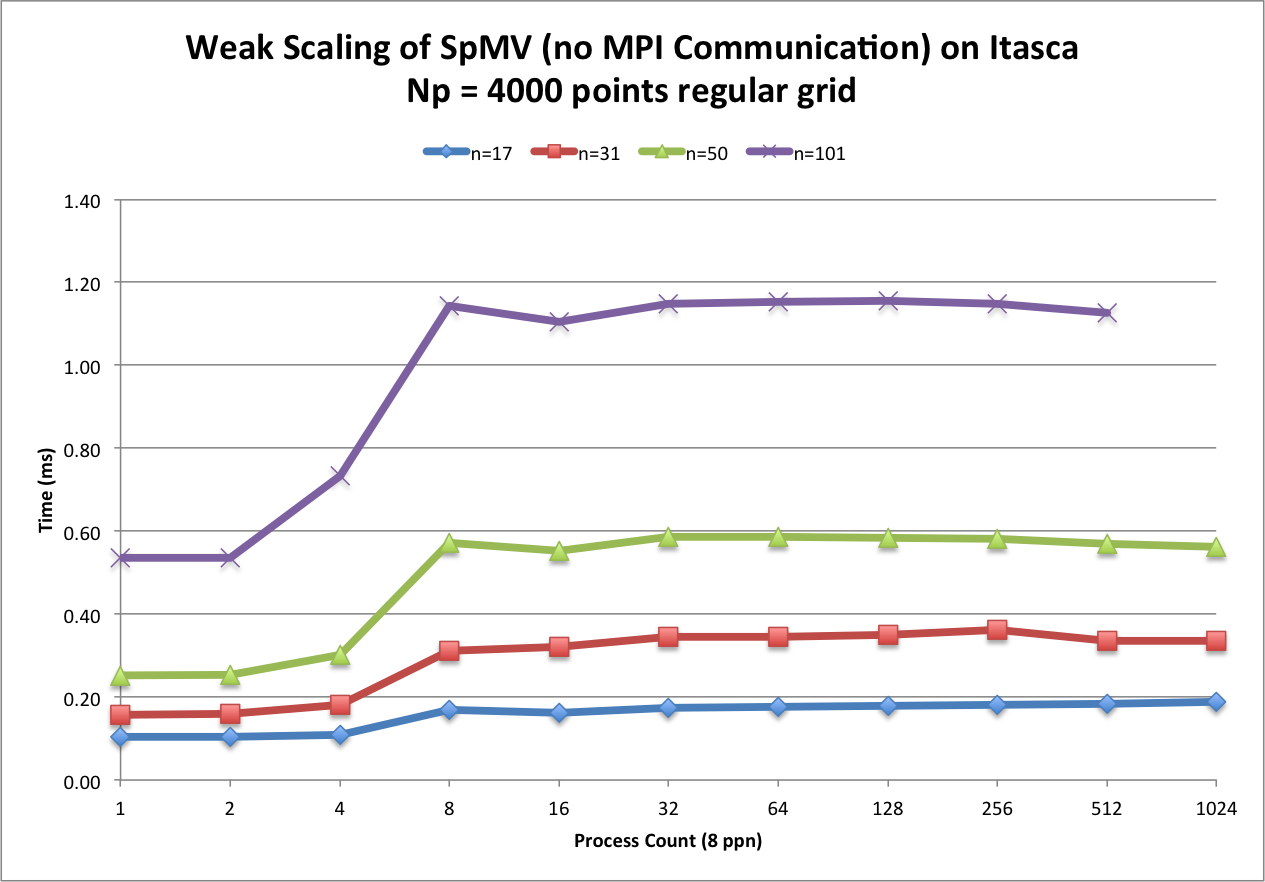
\includegraphics[width=\textwidth]{performance_content/scaling/weak_scaling_np4000_regular_spmvOnly.png}
\caption{SpMV only}
\label{fig:weak_scaling_spmv_only_alltoallv_all_stencils}
\end{subfigure}
\caption{Weak scaling of the SpMV. Increasing time for the SpMV reflects shared memory contention for processes on the same compute node (i.e., $p\leq 8$). Poor weak scaling is the result of growing communication times. }
\end{figure}


\subsection{Improvements}


Figure~\ref{fig:mpi_tuning} illustrates a progression of improvements made in effort to flatten the weak scaling curves from Figure~\ref{fig:weak_scaling_comm_only_alltoallv_all_stencils}. Each tile of Figure~\ref{fig:mpi_tuning} is a timeline for the distributed SpMV. Vertical bars separate the SpMV in focus from execution of the next and last SpMV. Our implementation does not assume a global barrier before starting the next iteration, so load balancing is essential to limit wait times between processors. Operations are concurrent from top to bottom within each tile, and the top-most operations are launched first.

%The distributed GPU implementation in Chapter~\ref{chap:multigpu_rbffd} is based on the collective in Figure~\ref{fig:overlap_cpu}. 

\begin{figure} 
\centering
\begin{subfigure}{0.48\textwidth}
\centering
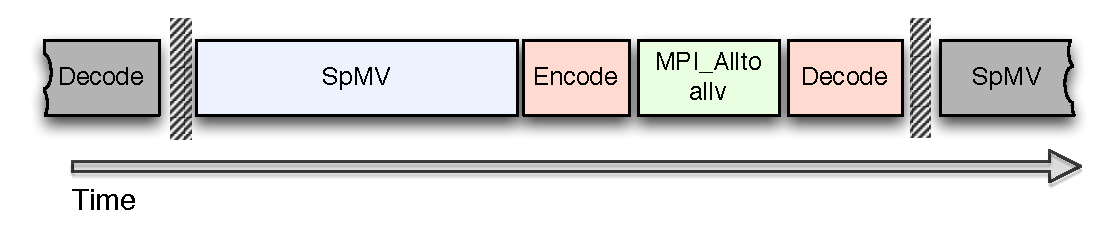
\includegraphics[width=\textwidth]{../figures/omnigraffle/AlltoallvCPU.pdf}
\caption{MPI\_Alltoallv}
\label{fig:alltoallv_cpu}
\end{subfigure}
\begin{subfigure}{0.48\textwidth}
\centering
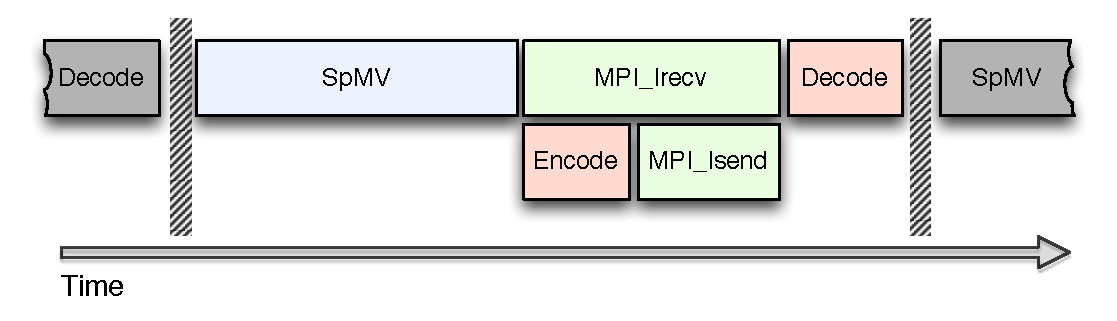
\includegraphics[width=\textwidth]{../figures/omnigraffle/IsendIrecvCPU.pdf}
\caption{MPI\_Isend/MPI\_Irecv}
\label{fig:isendirecv_cpu}
\end{subfigure}
\begin{subfigure}{0.48\textwidth}
\centering
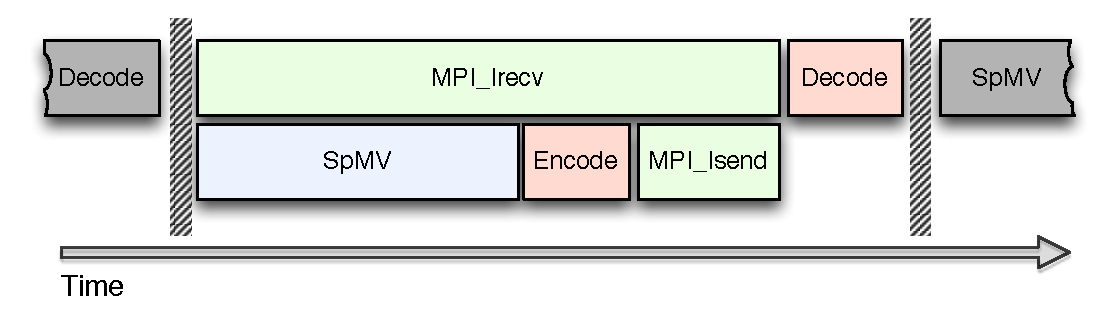
\includegraphics[width=\textwidth]{../figures/omnigraffle/IsendPreIrecvCPU.pdf}
\caption{Post an MPI\_Irecv before SpMV (``Pre-Recv")}
\label{fig:preirecv_cpu}
\end{subfigure}
\begin{subfigure}{0.48\textwidth}
\centering
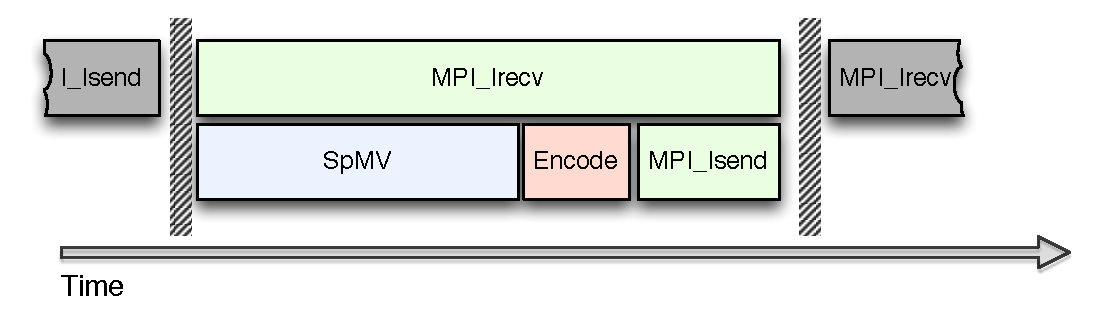
\includegraphics[width=\textwidth]{../figures/omnigraffle/NoDecode.pdf}
\caption{No Decode}
\label{fig:no_decode_cpu}
\end{subfigure}
\begin{subfigure}{0.48\textwidth}
\centering
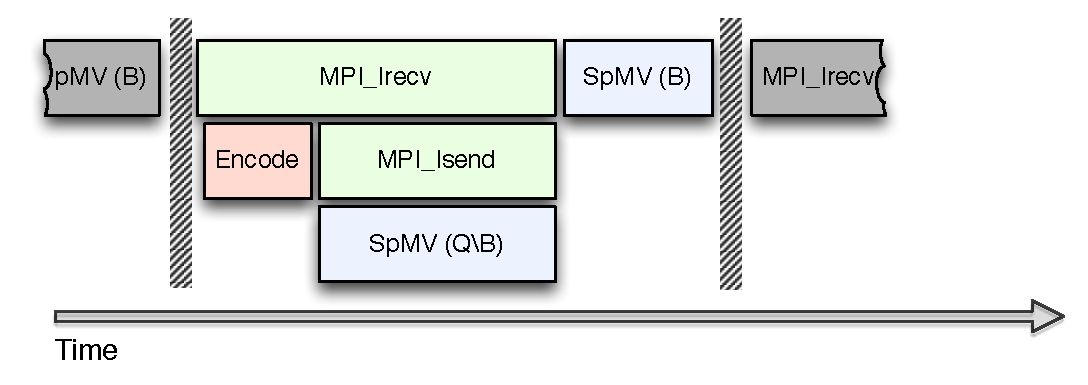
\includegraphics[width=\textwidth]{../figures/omnigraffle/OverlapCPU.pdf}
\caption{Overlapping SpMV and Communication}
\label{fig:overlap_cpu}
\end{subfigure}
\caption{MPI tuning steps to scale from 10 processors in \cite{BolligFlyerErlebacher2012} to 1024 processors here. Each horizontal timeline indicates the order of operations for a single distributed SpMV (i.e., between vertical bars). } 
\label{fig:mpi_tuning}
\end{figure}


Tuning occurred as follows for the $n=50$ node stencil case and $N_p=4000$ nodes per process:  
\begin{enumerate} 
\item The entire SpMV for $\setCenters$ is executed, followed by a blocking MPI\_Alltoallv collective (Figure~\ref{fig:alltoallv_cpu}). This is the baseline discussed above.
\item The MPI\_Alltoallv is replaced by non-blocking MPI\_Isend/MPI\_Irecv (Figure~\ref{fig:isendirecv_cpu}). This avoids unnecessary overhead in zero-byte message handling. 
\item MPI\_Irecv is issued \emph{before} starting the SpMV to ensure MPI\_Isends have pending connections when ready (Figure~\ref{fig:preirecv_cpu}). Posting the non-blocking receives early helps to hide some load balancing issues. 
\item Based on the assumption that elements of $\setDepend$ are sorted contiguous by neighboring process, the entire decode process is skipped (Figure~\ref{fig:no_decode_cpu}). 
\item MPI\_Irecv and MPI\_Isend are issued before computing the SpMV for set $\setCenters \backslash \setBoundary$. MPI\_Isend is non-blocking so the SpMV for $\setCenters \backslash \setBoundary$ starts before communication is complete. A barrier at the end of the first SpMV waits for communication to finish before launching the second SpMV on $\setBoundary$. This hides some cost of communication behind computation on the CPU (Figure~\ref{fig:overlap_cpu}). This collective is the basis for distributed GPU computing approach in Chapter~\ref{chap:multigpu_rbffd}.
\end{enumerate}

\noindent Weak scaling for each case is presented in Figure~\ref{fig:compare_weak_scaling_n50}. The gap between MPI\_Alltoallv (blue) and the basic MPI\_Isend/MPI\_Irecv (red) in Figure~\ref{fig:compare_weak_scaling_n50} nicely captures the substantial loss of time due to zero-byte message tests. Posting MPI\_Irecv before the SpMV (see the green line) shows moderate improvement for large $p$, and reflects that the load balancing of the test is getting worse. At $p=1024$ processes the overlapping CPU approach is 2.8x faster than the baseline. Although its scaling is not ideal, overlapping the SpMV and communication does represent a significant improvement over the original MPI\_Alltoallv. %At $p=1024$ the overlapped communication and computation is 
%TODO: what percentage overlapped? diff the comm time and SpMV1 time.

In similar fashion Figure~\ref{fig:compare_strong_scaling_n50} shows strong scaling for each of the collectives. Differences in curves are difficult to discern except for $p \leq 16$ and $p = 1024$. Starting with the latter case, observe that the trend of near linear scaling for the overlapping collective persists at $p=1024$ rather than bottoming-out in the fashion of MPI\_Alltoallv. 

For small $p$ the MPI\_Alltoallv is up to 2x faster than MPI\_Isend/MPI\_Irecv variants. For $p\leq8$ it is safe to assume MPI\_Alltoallv makes better use of local shared memory to communicate within the same node. Beyond $p=8$, the collective most likely improves on MPI\_Isend/MPI\_Irecv by optimally packing messages or even breaking large messages into smaller pieces. Its also possible to some extent for the collective to adjust to the network topology. Duplicating those optimizations for the overlapped CPU collective is left for future work. Until then, RBF-FD in distributed CPU environments like Itasca should assume the use of MPI\_Alltoallv collective for $p \leq 16$ and the overlapped MPI\_Isend/MPI\_Irecv in all other cases. 

\subsection{All Stencil Summary}



\begin{figure}
\centering
\begin{subfigure}[t]{0.48\textwidth}
\centering
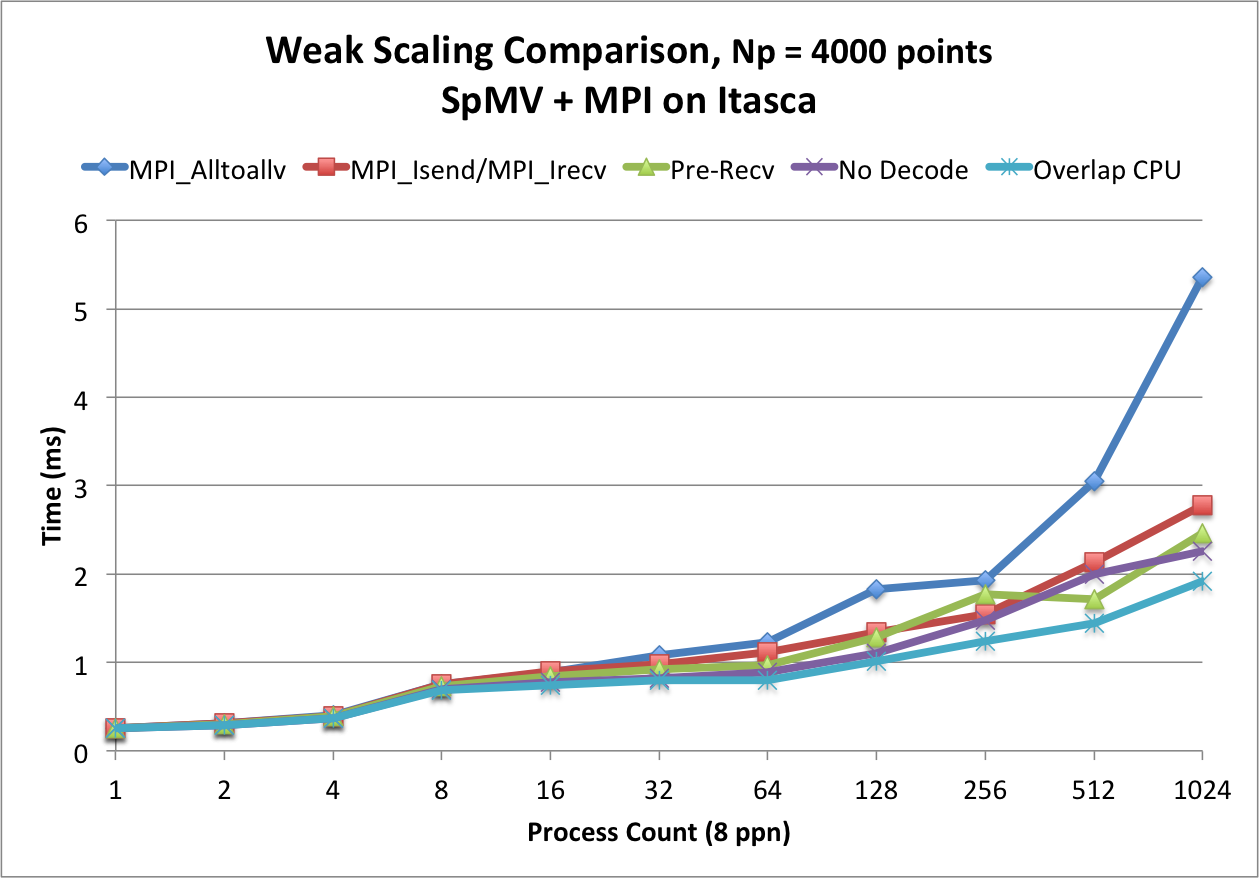
\includegraphics[width=\textwidth]{performance_content/scaling/weak_scaling_np4000_compare_SpMV_and_comm_n50.png}
\caption{Weak scaling comparison for $n=50$ and $N_p = 4000$ on a 3D regular grid with maximum resolution $N=4096000$ on Itasca.}
\label{fig:compare_weak_scaling_n50}
\end{subfigure}
\quad
\begin{subfigure}[t]{0.48\textwidth}
\centering
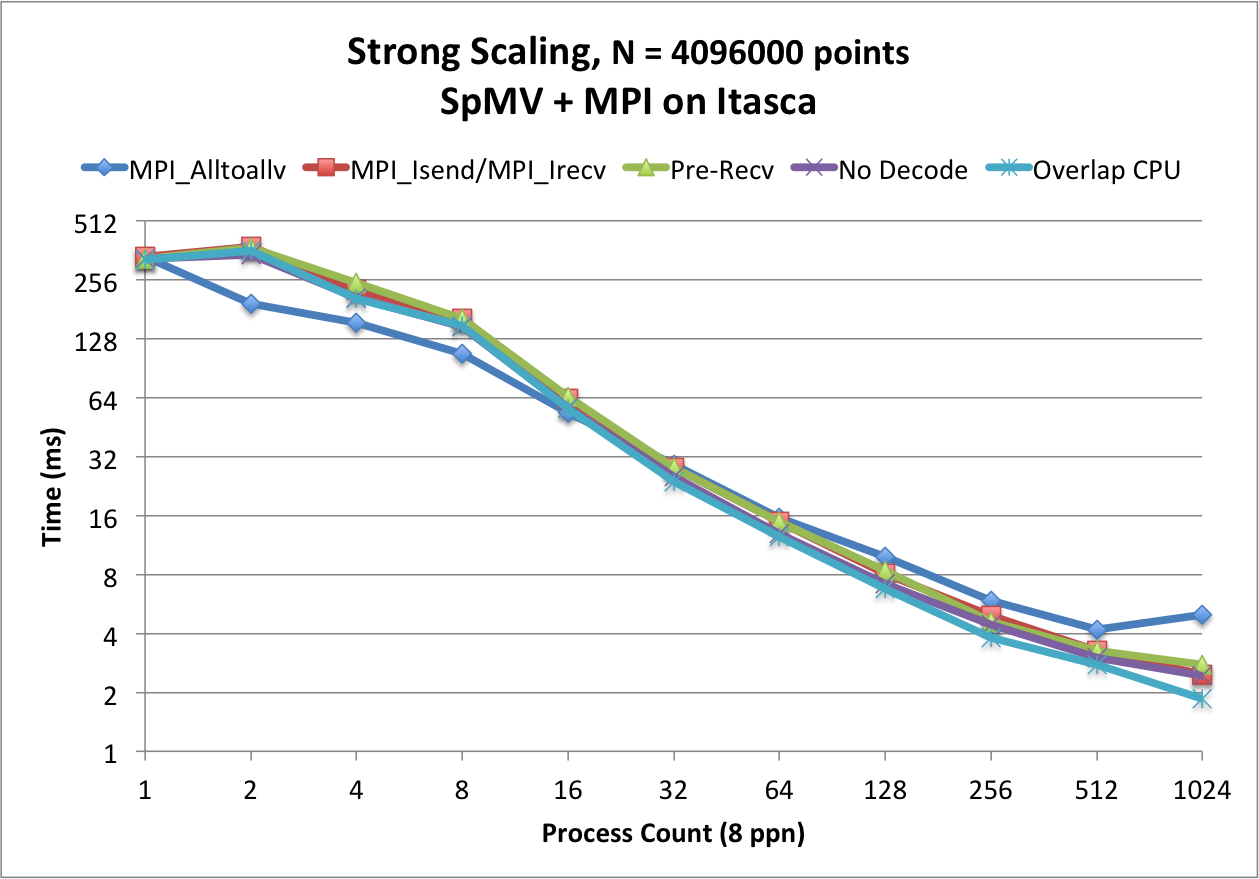
\includegraphics[width=\textwidth]{performance_content/scaling/strong_scaling_4M_compare_SpMV_and_comm_n50.png}
\caption{Strong scaling comparison for $n=50$ and $N = 4096000$ on a 3D regular grid on Itasca.}
\label{fig:compare_strong_scaling_n50}
\end{subfigure}
\caption{Weak and Strong Scaling Improvements}
\end{figure}

Figures~\ref{fig:compare_weak_scaling_all_stencils} and \ref{fig:compare_strong_scaling_all_stencils} demonstrate the scaling for the overlapped communication and computation and various stencil sizes ($n=17,31,50,101$). 

Figure~\ref{fig:compare_weak_scaling_all_stencils} shows that degradation in weak scaling starts at smaller $p$ as the stencil size, $n$, grows. This is attributed---at least in part---to the proportional increase in the number of ghost node dependencies per partition sent/received. Based on the comparison in \S~\ref{sec:load_balance}, the ratio of ghost node counts was found to be $\frac{\min N_r}{\max N_r} = 0.39$ for $p=1024$ and $n=17$. The low ratio points to imbalanced communication loads as one cause for communication increase. 
This may be a limitation in METIS when partitioning domains for large $p$. If so, future work may be able to improve balancing with other graph partitioning methods. 

\begin{figure}
\centering
\begin{subfigure}{0.48\textwidth}
\centering
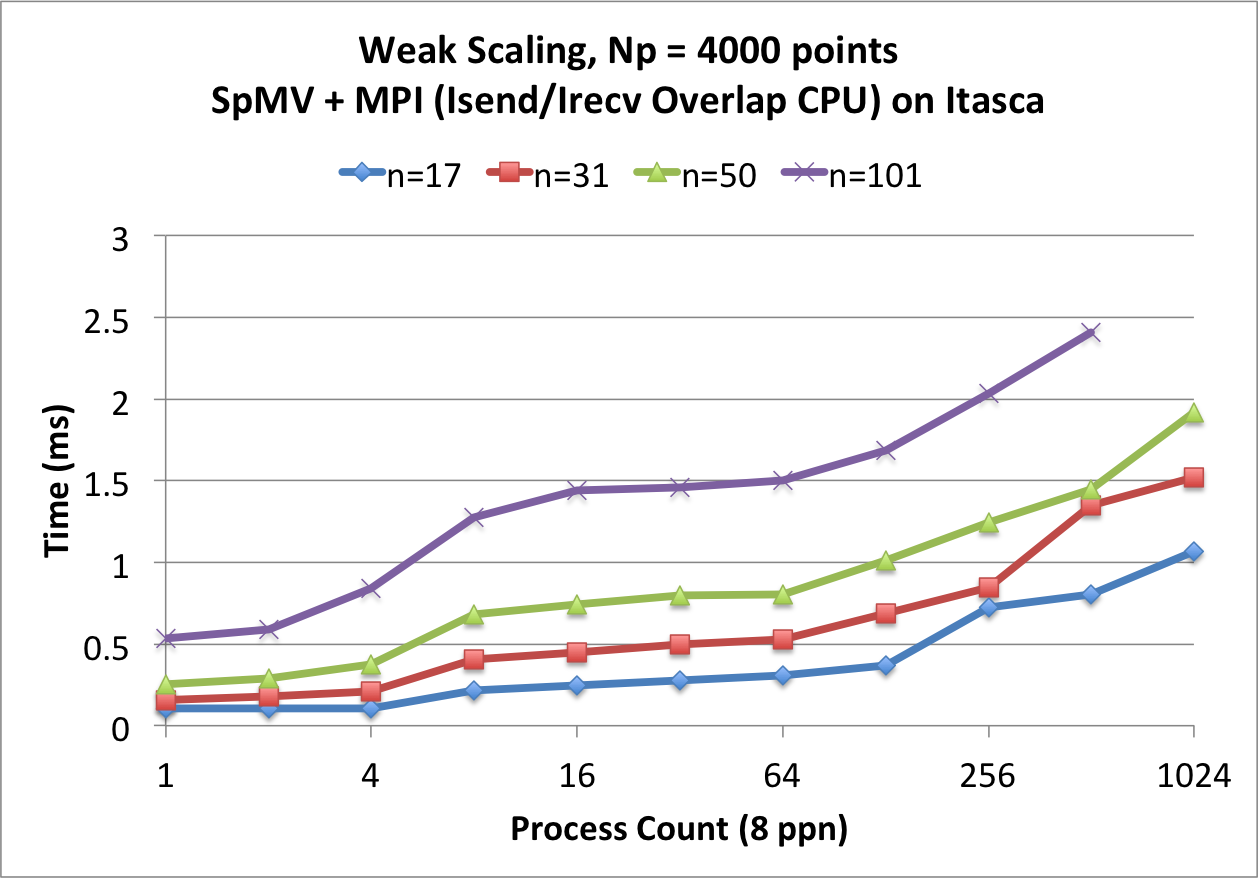
\includegraphics[width=\textwidth]{performance_content/scaling/weak_scaling_np4000_overlap_cpu_SpMV_and_comm_all_stencils.png}
\caption{Weak Scaling (All Stencils)}
\label{fig:compare_weak_scaling_all_stencils}
\end{subfigure}
\begin{subfigure}{0.48\textwidth}
\centering
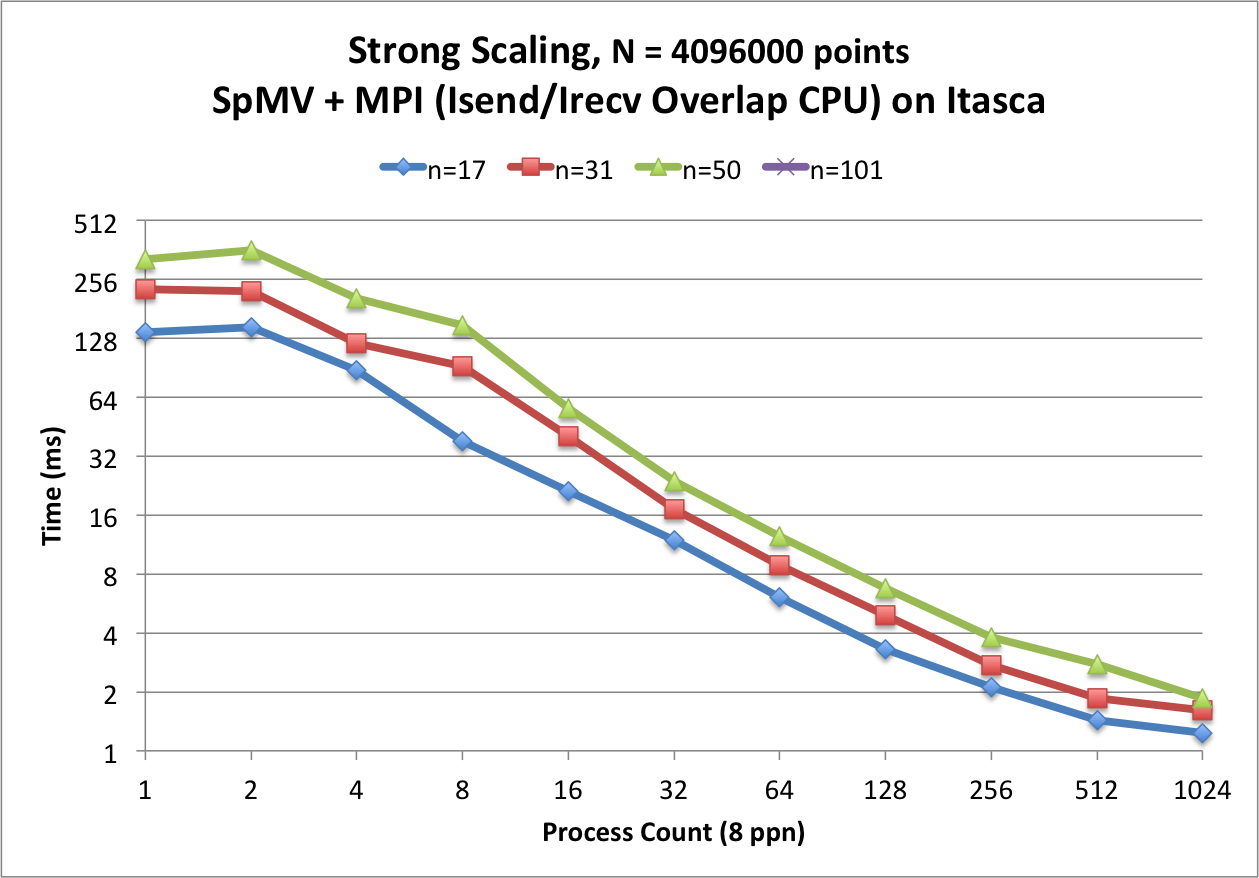
\includegraphics[width=\textwidth]{performance_content/scaling/strong_scaling_4M_overlap_cpu_SpMV_and_comm_all_stencils.png}
\caption{Strong Scaling (All Stencils)}
\label{fig:compare_strong_scaling_all_stencils}
\end{subfigure}
\caption{Weak and Strong scaling for various stencil sizes ($n=17, 31, 50, 101$). } 
\label{fig:weak_scaling_all_stencils}
\end{figure}


\begin{figure}
\centering
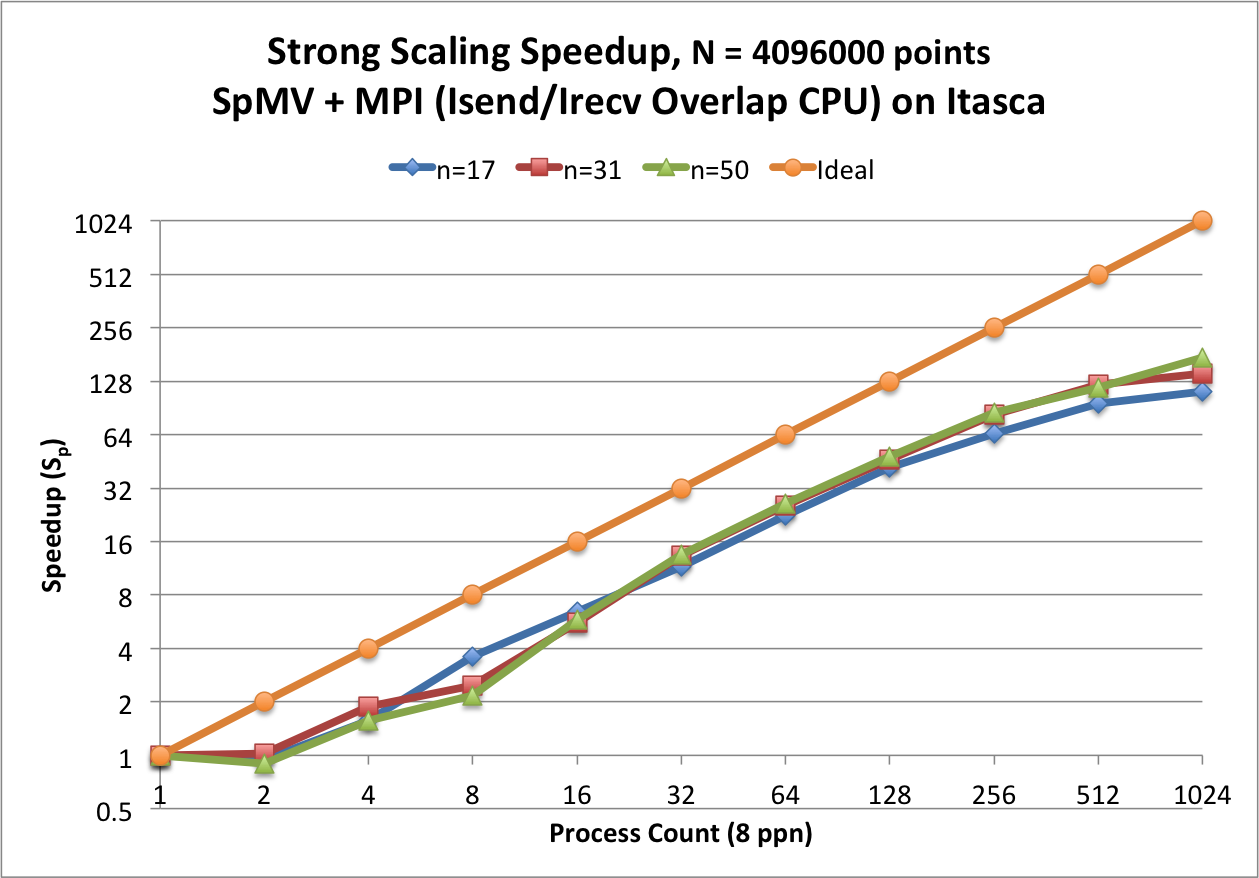
\includegraphics[width=0.5\textwidth]{performance_content/scaling/strong_scaling_speedup_4M_overlap_cpu_SpMV_and_comm_all_stencils.png}
\caption{Strong Scaling Speedup ($S_p = \ ^{t_{1}}/_{t_p}$)}
\label{fig:compare_strong_scaling_speedup_all_stencils}
\end{figure}


Figure~\ref{fig:compare_weak_scaling_all_stencils} demonstrates fair strong scaling for the implementation even though all three cases taper off toward the end. Figure~\ref{fig:compare_strong_scaling_speedup_all_stencils} presents the strong scaling in turns of speedup. Here we see that, after an initial slow-down due to MPI\_Isend/MPI\_Irecv, the implementation scales linearly up to $p=256$.



%By sampling the time between the start of the $\setCenters \backslash \setBoundary$ SpMV launch and the finish of the $\setBoundary$ SpMV kernel, one gets an approximation to $t_{SpMV}$, the total time spent computing the SpMV. Likewise the time between MPI\_Irecv and an MPI\_Waitall at the end of the $\setCenters \backslash \setBoundary$ SpMV gives the time spent in communication, $t_{Comm}$. Note that $t_{Comm}$ includes the encoding time. Figure~\ref{fig:compare_strong_scaling_comm_only_all_stencils} subtracts the $t_{Comm}$ and $t_{SpMV}$ to get an idea of what percentage of the original ti gives an idea of how much overlap hides communication. 
%


\begin{figure}
\centering
\begin{subfigure}{0.48\textwidth}
\centering
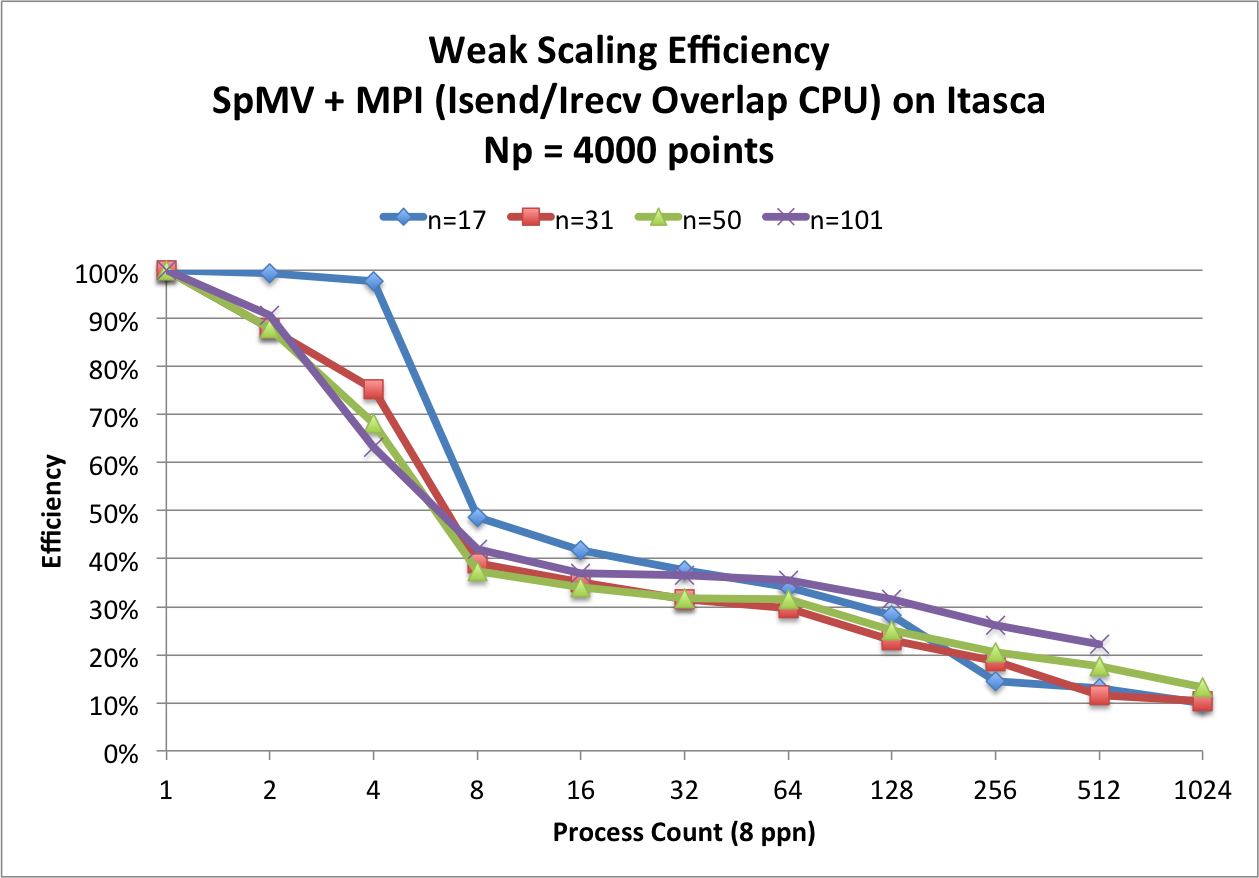
\includegraphics[width=\textwidth]{performance_content/scaling/weak_scaling_efficiency_np4000_overlap_cpu_SpMV_and_comm_all_stencils.png}
\caption{Weak Scaling Efficiency $E_p = \ ^{t_1}/_{t_p}$}
\label{fig:compare_weak_scaling_efficiency_all_stencils}
\end{subfigure}
\begin{subfigure}{0.48\textwidth}
\centering
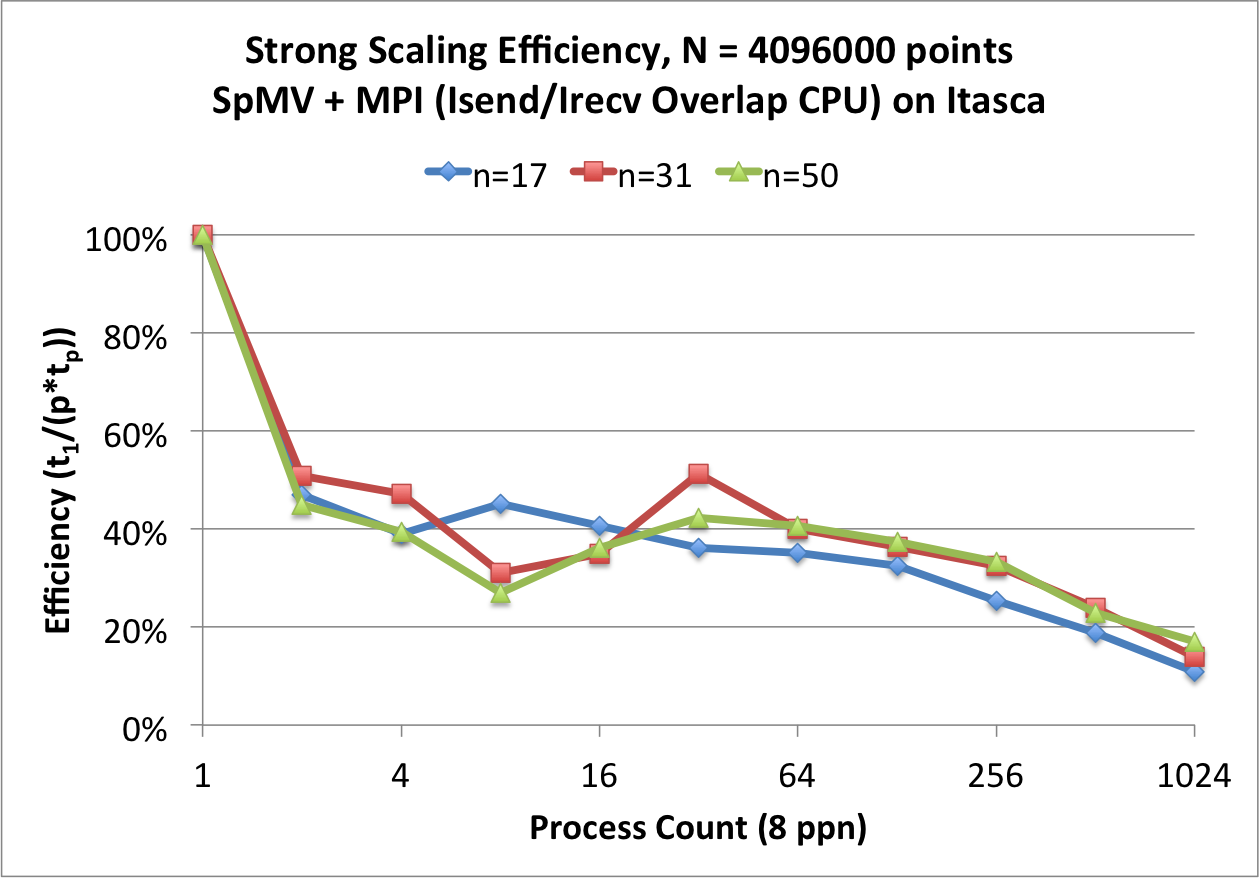
\includegraphics[width=\textwidth]{performance_content/scaling/strong_scaling_efficiency_4M_overlap_cpu_SpMV_and_comm_all_stencils.png}
\caption{Strong Scaling Efficiency ($E_p = \ ^{t_{1}}/_{p*t_p} $)}
\label{fig:compare_strong_scaling_efficiency_all_stencils}
\end{subfigure}
\caption{Scaling efficiency for various stencil sizes ($n=17, 31, 50, 101$) on a regular grid with $N_p$ maximum resolution $N=4096000$ on Itasca. } 
\label{fig:scaling_efficiency}
\end{figure}


For comparison with related work, and to assess how well the implementation utilizes hardware, we provide weak and strong scaling efficiencies in Figures~\ref{fig:compare_weak_scaling_efficiency_all_stencils} and \ref{fig:compare_strong_scaling_efficiency_all_stencils}. Efficiency can have multiple definitions, but is always expressed as a percentage of linear scaling with 100\% as ideal. Lower percentages indicate under-utilization of parallelism due to communication overhead or other issues.  Weak Scaling Efficiency is calculated as: 
\begin{align*}
E_p = \ ^{t_1}/_{t_p} * 100\%
\end{align*}
where $t_1$ is the execution time on 1 processor and $t_p$ is the time on $p$ processors.
Strong Scaling Efficiency is: 
\begin{align*}
E_p = \ ^{t_{1}}/_{(p*t_p)} * 100\%.
\end{align*}
Figures~\ref{fig:compare_weak_scaling_efficiency_all_stencils} and \ref{fig:compare_strong_scaling_efficiency_all_stencils} show our distributed RBF-FD achieves about 30\% to 40\% parallel efficiency in strong and weak cases for $p \leq 128$. At $p=1024$ strong and weak scaling converge to a little over 15\% efficiency. 

%TODO: Strong scaling efficiency for $p=128$ is at 33\% for $n=17$ and 37\% for $n=50$. A similar efficiency of 36\% was stated by the PetRBF implementation \cite{Yokota2010} for the Cray XT4. 

\begin{figure}
\centering
\begin{subfigure}{0.48\textwidth}
\centering
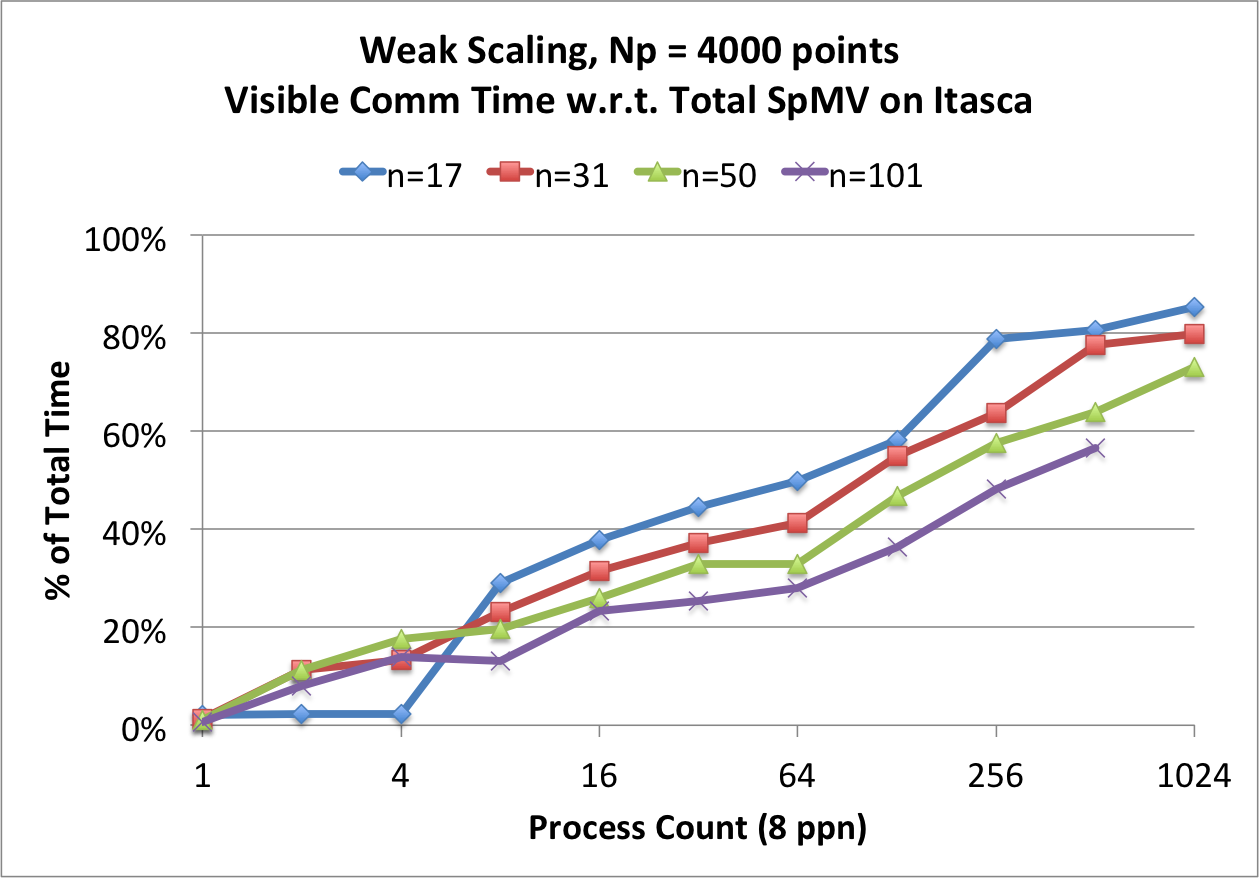
\includegraphics[width=\textwidth]{performance_content/scaling/weak_scaling_comm_only_np4000_overlap_cpu_SpMV_and_comm_all_stencils.png}
\caption{Weak Scaling}
\label{fig:compare_weak_scaling_unoverlapped_comm_all_stencils}
\end{subfigure}
\begin{subfigure}{0.48\textwidth}
\centering
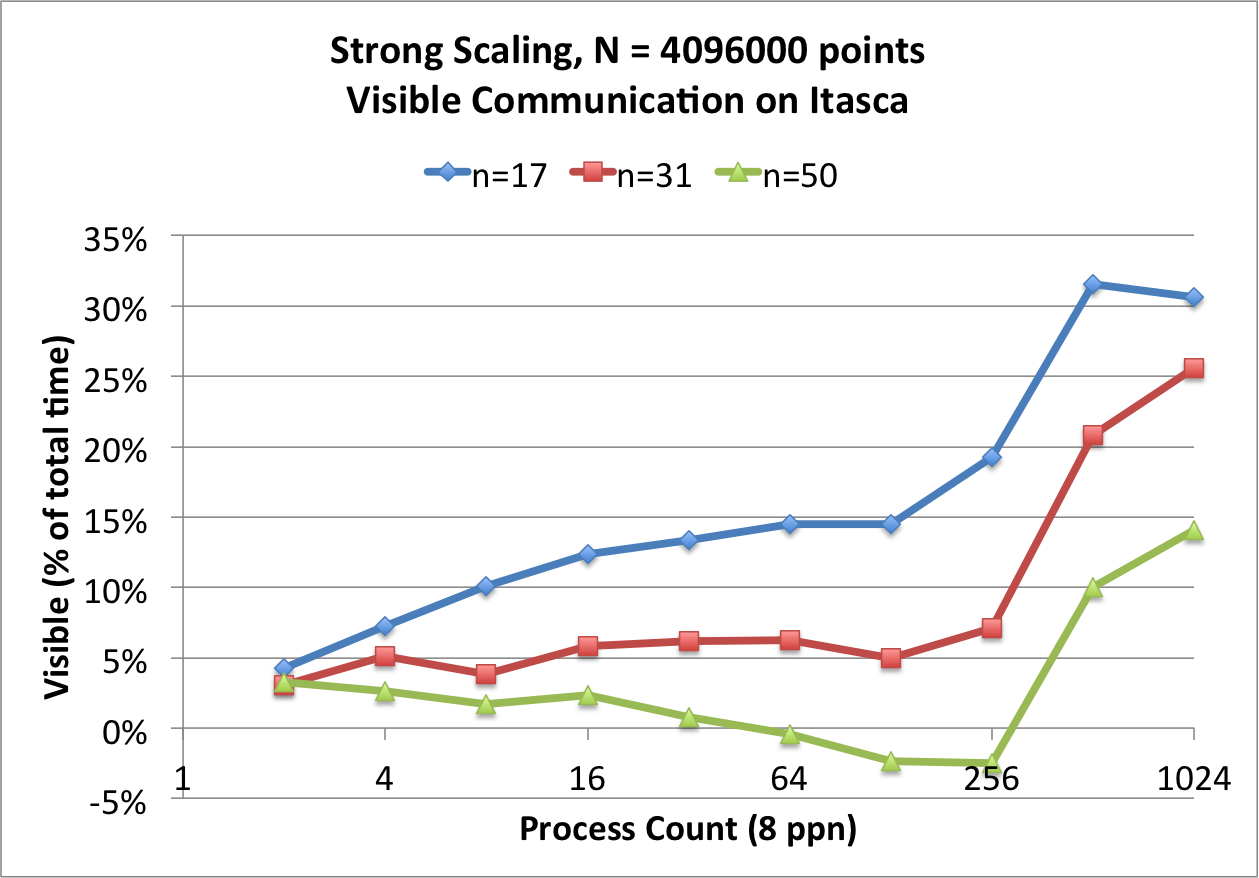
\includegraphics[width=\textwidth]{performance_content/scaling/strong_scaling_comm_only_4M_overlap_cpu_SpMV_and_comm_all_stencils.png}
\caption{Strong Scaling}
\label{fig:compare_strong_scaling_unoverlap_comm_all_stencils}
\end{subfigure}
\caption{Visible communication with respect to total SpMV Time. Lower is better.}
\label{fig:visible_comm}
\end{figure}


Figures~\ref{fig:compare_weak_scaling_unoverlapped_comm_all_stencils} and \ref{fig:compare_strong_scaling_unoverlap_comm_all_stencils}  quantify the overhead in communication for all weak and strong scaling test cases. Both figures show the percentage of \emph{visible communication time}, $t_{vis}$, during an iteration of the distributed SpMV. The visible time is defined as: 
\begin{align*}
t_{Vis} = \ ^{(t_{Comm} - t_{SpMV 1}}) /_{t_{Total}}
\end{align*}
where $t_{Vis}$ is the subset of time between the first MPI\_Irecv post and the start of the first SpMV (for $\setCenters \backslash \setBoundary$). Any communication hidden by the first SpMV is subtracted off $t_{Comm}$ with $t_{SpMV 1}$, the time spent computing.

The local minima in  Figure~\ref{fig:compare_strong_scaling_unoverlap_comm_all_stencils} reveal an optimal choice of $p$ by stencil size for overlapping communication and computation. Note that the minima at $p=8$ for $n=17$, and $p=32$ for $n=31$ and $50$ correspond to strong scaling efficiency peaks in Figure~\ref{fig:compare_strong_scaling_efficiency_all_stencils}.

 For weak scaling, the constant SpMV computation time (and constant overlap) means the linear trend in Figure~\ref{fig:compare_weak_scaling_unoverlapped_comm_all_stencils}  is purely growth in communication time with respect to $p$. Possible causes include (but are not limited to): 
\begin{itemize}
\item \emph{Worsening load balance}. As previously mentioned, METIS may be incapable of partitioning the domain optimally.
\item \emph{Network contention}. As the number of processes scale the increasing network traffic is expected to slow MPI globally.  
\item \emph{Improperly padded or aligned messages}. MPI, like any other software, operates most efficiently when data is properly aligned and messages have the right size. 
\end{itemize}
All three of these concerns will be investigated as part of future work. 

%
%As an aside, some benchmark on Spear highlight the imbalanced workloads on processors. Excessive wait times on MPI collectives meant that processes were not entering communication stages at similar times. In response launched a new effort to load-balance and tune MPI for a large number of processes.


\section{Conclusion}

This chapter covered the design and tuning of the first distributed RBF-FD implementation for CPU and GPU clusters. The implementation was demonstrated to be scalable with 30\% to 40\% parallel efficiency on 128 processors of the Itasca HPC (CPU-only) cluster at the University of Minnesota given a problem size of $N=4096000$ nodes and stencil sizes between $n=17$ and $n=50$. 

A number of optimizations reduce communication times and increase scalability beyond the results in our first paper, \cite{BolligFlyerErlebacher2012}. Starting with an MPI\_Alltoallv collective, the tuning effort ultimately leads to a scheme which overlaps communication and computation on the CPU. Chapter~\ref{chap:multigpu_rbffd} extends this collective to overlap with computation on GPUs. 

Our implementation leverages METIS for general domain decomposition and load balancing. Individual processes do not require a full mapping between RBF nodes and CPUs. Instead, processes assemble and operate on local linear systems for their subdomains. Communication between processes is limited to nearest-neighbor or all-to-subset collectives based on the intersection of subdomains. 
		



\chapter{Distributed GPU SpMV (incomplete)}
\label{chap:multigpu_rbffd}


\cite{Lawlor2009}
%TODO: \cite{Goeddeke2009} \cite{Erez2007}

Distributing SpMV across multiple GPUs poses a new problem: as previous mentioned, the data sent and received via MPI collectives must be copied from device to host and vice-versa. To amortize this cost we introduce a novel overlapping algorithm to hide the cost of communication behind the cost of a concurrent SpMV on the GPU. 


Petascale computing centers around the world are leveraging GPU accelerators to achieve peak performance. In fact, many of today's high performance computing installations boast significantly more GPU accelerators than CPU counterparts. The Keeneland project is one such example, currently with 240 CPUs accompanied by 360 NVidia Fermi class GPUs with at least double that number expected by the end of 2012 \cite{Vetter2011}. 

Such throughput oriented architectures require developers to decompose problems into thousands of independent parallel tasks in order to fully harness the capabilities of the hardware. To this end, a plethora of research has been dedicated to researching algorithms in all fields of computational science. Of interest to us are methods for atmospheric- and geo-sciences. 


Similar approaches to overlapping communication and computation can be found in \cite{Schubert2011} and \cite{Thibault2009}.

When operating on multiple GPUs we avoid the copy-out or decode phase by requiring that the local ordering of nodes sort the set $\setDepend$ by the rank of the process sending each node. This way, when the MPI collective finishes and all values arrive contiguous by provider, the data can be copied directly to the GPU without reordering.

\section{Overlapping with the GPU}

Overlapping communication and computation with the GPU is made possible with two levels of asynchronous commands: 
\begin{itemize} 
\item \emph{Non-blocking MPI}. The MPI\_Isend/MPI\_Irecv routines are used to post communication and immediately return the main thread to computation. 
\item \emph{Asynchronous GPU Queues}. Two OpenCL queues are utilized to send commands to the GPU. 
\end{itemize}

 
\begin{figure} 
\centering
\begin{subfigure}{0.48\textwidth}
\centering
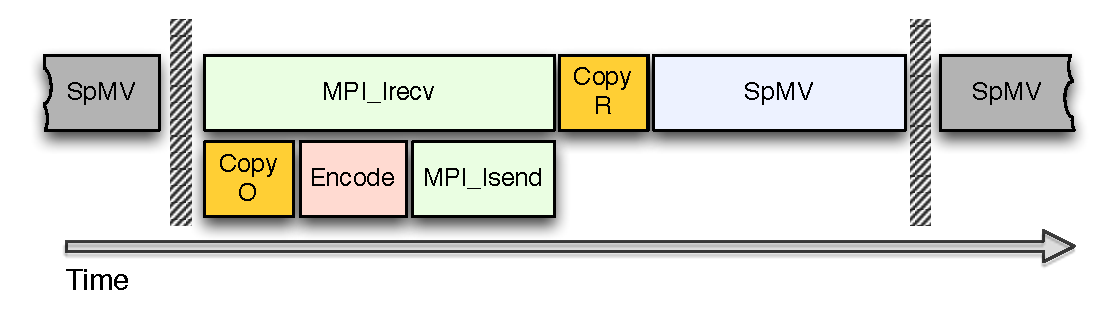
\includegraphics[width=\textwidth]{../figures/omnigraffle/GPU_IsendIrecv.pdf}
\caption{GPU and MPI\_Isend/MPI\_Irecv (Non-Overlapping)}
\label{fig:isendirecv_gpu}
\end{subfigure}
\quad
\begin{subfigure}{0.48\textwidth}
\centering
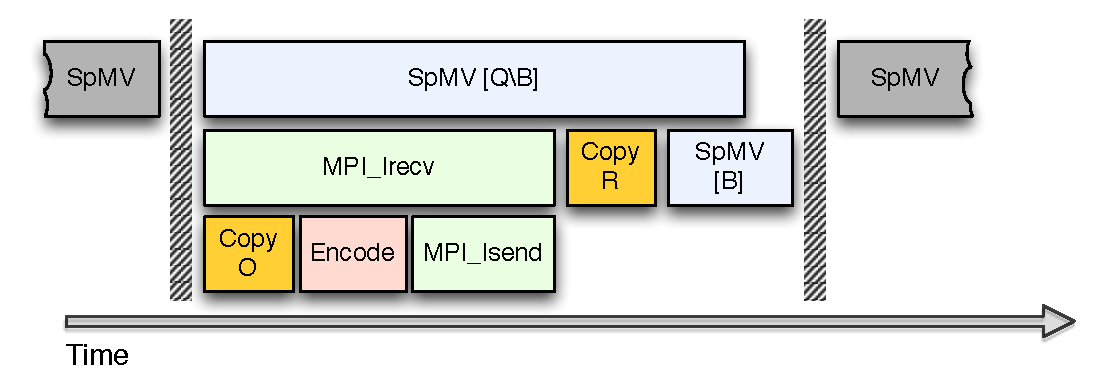
\includegraphics[width=\textwidth]{../figures/omnigraffle/GPU_OverlapGPU.pdf}
\caption{GPU and MPI\_Isend/MPI\_Irecv (Overlapping)}
\label{fig:overlap_gpu}
\end{subfigure}
\caption{Overlapping GPU kernels with CPU managed communication. } 
\label{fig:gpu_mpi_tuning}
\end{figure}

\section{Scaling}
We scale the SpMV across the GPUs on Cascade.


By comparing benchmarks from the unoverlapped and overlapped GPU cases, we get the speedup in using the overlapped solution. Any reduction in time is evidence of overlap. 

Calculating the percentage reduction is useful to consider. The benchmarks are not complete (i.e., the actual time to compute SpMV1 is unknown). However, the time spent in non-SpMV related tasks (e.g., data transfer, encoding, and communication) is known from the unoverlapped case. Therefore, given the time for the overlapped SpMV case, we can calculate the amount of overlap as 

%
%\begin{align}
%t_{nooverlap, SpMV} - (t_{overlap, tot} - t_{overlap, nonSpMV}) \\
%t_{overlap} = t_{overlap} - (t_{comm} + t_{en} + t_{R} + t_{O})  \\
%(SpMV whole) - (SpMV2) \approx (SpMV1) \\
%If (SpMV1) > (Comm + SpMV2) 
%\end{align}
%% percent reduction is useful to tell overlap. e.g., if we reduce by 25% and the 
%
%Right, so the time from the start of comm to the end of the SpMV2 should be 
%
%\begin{table}[h]
%\centering
%\caption{GFLOP/s observed for distributed ELL SpMV on Cascade's M2070 GPUs without overlapping communication and GPU kernels.}
%\label{tbl:cascade_m2070_nooverlap}
%\begin{tabular}{c|c|c|c|c|c|c}
%Compute Nodes   &   PPN   &   n=17   &   n=31   &   n=50   &   n=101   \\ \hline
%1   &   1   &   8.4   &   8.4   &   8.9   &      \\
%2   &   1   &   6.1   &   6.8   &   6.4   &   7.6   \\
%4   &   1   &   6.9   &   9.1   &   10.3   &   13.3   \\
%8   &   1   &   12.1   &   14.6   &   12.1   &   23.0   \\ \hline
%1   &   2   &   3.4   &   4.1   &   3.7   &   4.2   \\
%2   &   2   &   4.4   &   5.4   &   6.5   &   8.1   \\
%4   &   2   &   11.1   &   9.3   &   9.9   &   14.2   \\
%8   &   2   &   15.9   &   15.4   &   22.2   &   23.9   \\ \hline
%1   &   4   &   3.3   &   4.4   &   5.1   &   5.5   \\
%2   &   4   &   8.3   &   7.6   &   9.5   &   11.0   \\
%4   &   4   &   12.4   &   12.9   &   18.7   &   18.0   \\
%8   &   4   &   17.4   &   28.4   &   28.0   &   37.4   
%\end{tabular}
%\end{table}


\begin{table}[h]
\centering
\caption{GFLOP/sec achieved by the distributed ELL SpMV on Cascade's M2070 GPUs, with MPI communication overlapping two GPU kernels. The SpMV computes derivatives over a 3D regular grid of size $N=4096000$ nodes (i.e., $160^3$). Data reflects various combinations of stencil sizes, number of compute nodes and number of processes per node (PPN). Quantities in parentheses denote the speedup factors achieved by the overlapping algorithm over the non-overlapping approach for identical combinations of compute nodes, PPN, stencil size, etc. }
\label{tbl:cascade_m2070_overlap}
\begin{tabular}{c|c|c|c|c|c|c}
 \multicolumn{2}{c}{ } & \multicolumn{4}{|c|}{Observed GFLOP/sec (Speedup over Non-overlapped)} \\  \hline
Compute Nodes   &   PPN  &   n=17   &   n=31   &   n=50   &   n=101   \\ \hline
1   &   1   &   8.5 (1.0x)   &   8.4 (1.0x)   &   13.2 (1.5x)   &      \\
2   &   1   &   13.8 (2.3x)   &   13.0 (1.9x)   &   9.0 (1.4x)   &   13.5 (1.8)   \\
4   &   1   &   13.1 (1.9x)   &   25.1 (2.8x)   &   24.6 (2.4x)   &   25.2 (1.9)   \\
8   &   1   &   24.5 (2.0x)   &   33.2 (2.3x)   &   41.2 (3.4x)   &   53.6 (2.3x)   \\ \hline
1   &   2   &   11.3 (3.4x)   &   12.2 (3.0x)   &   12.1 (3.2x)   &   12.7 (3.0x)   \\
2   &   2   &   13.0 (3.0x)   &   22.9 (4.2x)   &   23.1 (3.6x)   &   53.5 (\textbf{6.6x})   \\
4   &   2   &   25.1 (2.3x)   &   37.8 (4.1x)   &   50.1 (5.0x)   &   24.5 (1.7x)   \\
8   &   2   &   35.8 (2.2x)   &   38.3 (2.5x)   &   59.6 (2.7x)   &   87.6 (3.7x)   \\ \hline
1   &   4   &   27.7 (\textbf{8.5x})   &   22.5 (\textbf{5.1x})   &   27.9 (\textbf{5.4x})   &   24.4 (4.4x)   \\
2   &   4   &   14.1 (1.7x)   &   32.0 (4.2x)   &   37.2 (3.9x)   &   50.8 (4.6x)   \\
4   &   4   &   19.6 (1.6x)   &   38.6 (3.0x)   &   57.0 (3.0x)   &   81.3 (4.5x)   \\
8   &   4   &   50.9 (2.9x)   &   61.6 (2.2x)   &   88.8 (3.2x)   &   130.8 (3.5x)  
\end{tabular} 
\end{table}

%1.0	1.0	1.5	#DIV/0!
%2.3	1.9	1.4	1.8
%1.9	2.8	2.4	1.9
%2.0	2.3	3.4	2.3
%3.4	3.0	3.2	3.0
%3.0	4.2	3.6	6.6
%2.3	4.1	5.0	1.7
%2.2	2.5	2.7	3.7
%8.5	5.1	5.4	4.4
%1.7	4.2	3.9	4.6
%1.6	3.0	3.0	4.5
%2.9	2.2	3.2	3.5

\subsection{Multiple Kernel Scheduling}
describe fermi's ability to schedule multiple kernels, what it means for our queues. Do we need multiple queues, or just one that is non-blocking. How do we indicate we are done communicating if there is no queue to add markers to? 


\section{HPC Spear Cluster} 
See Appendix for Spear data with MPI\_Alltoallv (no overlap). 
\section{Keeneland}

\subsection{Shared K20s}
The new Kepler K20s allow both concurrent kernel execution and dynamic parallelism. Dynamic parallelism is a means of scheduling new kernel launches from within an exist kernel. In order to support this feature,

K20s also support CUDA 5.5 which introduces MPI aware CUDA. The nvcc compiler now detects MPI calls and routes data movement directly from InfiniBand to the GPU memory rather than making a stop on the host memory. This is only possible with GPUDirect (direct memory addressing) and dynamic parallelism (to spawn an MPI process from a kernel). 

Features like MPI-CUDA will are unlikely to be available in OpenCL in the future. NVidia is no longer leading or distributing the OpenCL libraries with their driver. NVidia only plans to support the OpenCL spec v1.1.


\section{Future Work}

One of the problems with choosing to work in OpenCL is the fact that the standard offers the lowest common denominator of features from the various hardware vendors that support it. Many vendor specific features never make it into the language. 

Take for example GPUDirect, a technology introduced first CUDA v3.1 for NVidia hardware. GPUDirect allows direct access to GPU memory addresses from various sources including other GPUs. The technology allows GPUs to bypass copies to host memory en-route to another GPU on the same compute node. Combine GPUDirect with the new MPI aware features in CUDA v5.0 and data can pass directly from a GPU onto the infiniband fabric and up to another GPU \cite{NvidiaGPUMPI}. This type of feature may never be available in OpenCL. 




\ifstandalone
\bibliographystyle{plain}
\bibliography{merged_references}
\end{document}
\else
\expandafter\endinput
\fi

